\PassOptionsToPackage{unicode=true}{hyperref} % options for packages loaded elsewhere
\PassOptionsToPackage{hyphens}{url}
%
\documentclass[]{book}
\usepackage{lmodern}
\usepackage{amssymb,amsmath}
\usepackage{ifxetex,ifluatex}
\usepackage{fixltx2e} % provides \textsubscript
\ifnum 0\ifxetex 1\fi\ifluatex 1\fi=0 % if pdftex
  \usepackage[T1]{fontenc}
  \usepackage[utf8]{inputenc}
  \usepackage{textcomp} % provides euro and other symbols
\else % if luatex or xelatex
  \usepackage{unicode-math}
  \defaultfontfeatures{Ligatures=TeX,Scale=MatchLowercase}
\fi
% use upquote if available, for straight quotes in verbatim environments
\IfFileExists{upquote.sty}{\usepackage{upquote}}{}
% use microtype if available
\IfFileExists{microtype.sty}{%
\usepackage[]{microtype}
\UseMicrotypeSet[protrusion]{basicmath} % disable protrusion for tt fonts
}{}
\IfFileExists{parskip.sty}{%
\usepackage{parskip}
}{% else
\setlength{\parindent}{0pt}
\setlength{\parskip}{6pt plus 2pt minus 1pt}
}
\usepackage{hyperref}
\hypersetup{
            pdftitle={ELEMENTOS DE PROBABILIDAD E INFERENCIA ESTADÍSTICA},
            pdfauthor={Dr.~Jaime Lincovil C.},
            pdfborder={0 0 0},
            breaklinks=true}
\urlstyle{same}  % don't use monospace font for urls
\usepackage{color}
\usepackage{fancyvrb}
\newcommand{\VerbBar}{|}
\newcommand{\VERB}{\Verb[commandchars=\\\{\}]}
\DefineVerbatimEnvironment{Highlighting}{Verbatim}{commandchars=\\\{\}}
% Add ',fontsize=\small' for more characters per line
\usepackage{framed}
\definecolor{shadecolor}{RGB}{248,248,248}
\newenvironment{Shaded}{\begin{snugshade}}{\end{snugshade}}
\newcommand{\AlertTok}[1]{\textcolor[rgb]{0.94,0.16,0.16}{#1}}
\newcommand{\AnnotationTok}[1]{\textcolor[rgb]{0.56,0.35,0.01}{\textbf{\textit{#1}}}}
\newcommand{\AttributeTok}[1]{\textcolor[rgb]{0.77,0.63,0.00}{#1}}
\newcommand{\BaseNTok}[1]{\textcolor[rgb]{0.00,0.00,0.81}{#1}}
\newcommand{\BuiltInTok}[1]{#1}
\newcommand{\CharTok}[1]{\textcolor[rgb]{0.31,0.60,0.02}{#1}}
\newcommand{\CommentTok}[1]{\textcolor[rgb]{0.56,0.35,0.01}{\textit{#1}}}
\newcommand{\CommentVarTok}[1]{\textcolor[rgb]{0.56,0.35,0.01}{\textbf{\textit{#1}}}}
\newcommand{\ConstantTok}[1]{\textcolor[rgb]{0.00,0.00,0.00}{#1}}
\newcommand{\ControlFlowTok}[1]{\textcolor[rgb]{0.13,0.29,0.53}{\textbf{#1}}}
\newcommand{\DataTypeTok}[1]{\textcolor[rgb]{0.13,0.29,0.53}{#1}}
\newcommand{\DecValTok}[1]{\textcolor[rgb]{0.00,0.00,0.81}{#1}}
\newcommand{\DocumentationTok}[1]{\textcolor[rgb]{0.56,0.35,0.01}{\textbf{\textit{#1}}}}
\newcommand{\ErrorTok}[1]{\textcolor[rgb]{0.64,0.00,0.00}{\textbf{#1}}}
\newcommand{\ExtensionTok}[1]{#1}
\newcommand{\FloatTok}[1]{\textcolor[rgb]{0.00,0.00,0.81}{#1}}
\newcommand{\FunctionTok}[1]{\textcolor[rgb]{0.00,0.00,0.00}{#1}}
\newcommand{\ImportTok}[1]{#1}
\newcommand{\InformationTok}[1]{\textcolor[rgb]{0.56,0.35,0.01}{\textbf{\textit{#1}}}}
\newcommand{\KeywordTok}[1]{\textcolor[rgb]{0.13,0.29,0.53}{\textbf{#1}}}
\newcommand{\NormalTok}[1]{#1}
\newcommand{\OperatorTok}[1]{\textcolor[rgb]{0.81,0.36,0.00}{\textbf{#1}}}
\newcommand{\OtherTok}[1]{\textcolor[rgb]{0.56,0.35,0.01}{#1}}
\newcommand{\PreprocessorTok}[1]{\textcolor[rgb]{0.56,0.35,0.01}{\textit{#1}}}
\newcommand{\RegionMarkerTok}[1]{#1}
\newcommand{\SpecialCharTok}[1]{\textcolor[rgb]{0.00,0.00,0.00}{#1}}
\newcommand{\SpecialStringTok}[1]{\textcolor[rgb]{0.31,0.60,0.02}{#1}}
\newcommand{\StringTok}[1]{\textcolor[rgb]{0.31,0.60,0.02}{#1}}
\newcommand{\VariableTok}[1]{\textcolor[rgb]{0.00,0.00,0.00}{#1}}
\newcommand{\VerbatimStringTok}[1]{\textcolor[rgb]{0.31,0.60,0.02}{#1}}
\newcommand{\WarningTok}[1]{\textcolor[rgb]{0.56,0.35,0.01}{\textbf{\textit{#1}}}}
\usepackage{longtable,booktabs}
% Fix footnotes in tables (requires footnote package)
\IfFileExists{footnote.sty}{\usepackage{footnote}\makesavenoteenv{longtable}}{}
\usepackage{graphicx,grffile}
\makeatletter
\def\maxwidth{\ifdim\Gin@nat@width>\linewidth\linewidth\else\Gin@nat@width\fi}
\def\maxheight{\ifdim\Gin@nat@height>\textheight\textheight\else\Gin@nat@height\fi}
\makeatother
% Scale images if necessary, so that they will not overflow the page
% margins by default, and it is still possible to overwrite the defaults
% using explicit options in \includegraphics[width, height, ...]{}
\setkeys{Gin}{width=\maxwidth,height=\maxheight,keepaspectratio}
\setlength{\emergencystretch}{3em}  % prevent overfull lines
\providecommand{\tightlist}{%
  \setlength{\itemsep}{0pt}\setlength{\parskip}{0pt}}
\setcounter{secnumdepth}{5}
% Redefines (sub)paragraphs to behave more like sections
\ifx\paragraph\undefined\else
\let\oldparagraph\paragraph
\renewcommand{\paragraph}[1]{\oldparagraph{#1}\mbox{}}
\fi
\ifx\subparagraph\undefined\else
\let\oldsubparagraph\subparagraph
\renewcommand{\subparagraph}[1]{\oldsubparagraph{#1}\mbox{}}
\fi

% set default figure placement to htbp
\makeatletter
\def\fps@figure{htbp}
\makeatother

\usepackage{booktabs}
\usepackage[utf8]{inputenc}
\usepackage[spanish]{babel}
\selectlanguage{spanish}
\usepackage{amsthm}
\usepackage{graphicx}
\usepackage{pifont}
%\theoremstyle{plain} 
%\newtheorem{observacion}{Observación}
%\newtheorem{interpretacion}{Interpretación}
%\newtheorem{definition}{Definicion} 
%\newtheorem{ejem}{Ejemplos}
%\newtheorem{teo}{Teorema}
%\newtheorem{lema}{Lema}
\usepackage[]{natbib}
\bibliographystyle{apalike}

\title{ELEMENTOS DE PROBABILIDAD E INFERENCIA ESTADÍSTICA}
\author{Dr.~Jaime Lincovil C.}
\date{2021-01-28}

\usepackage{amsthm}
\newtheorem{theorem}{Teorema.}[chapter]
\newtheorem{lemma}{Lema.}[chapter]
\newtheorem{corollary}{Corolario.}[chapter]
\newtheorem{proposition}{Proposición.}[chapter]
\newtheorem{conjecture}{Conjetura.}[chapter]
\theoremstyle{definition}
\newtheorem{definition}{Definición.}[chapter]
\theoremstyle{definition}
\newtheorem{example}{Ejemplo.}[chapter]
\theoremstyle{definition}
\newtheorem{exercise}{Ejercicio.}[chapter]
\theoremstyle{remark}
\newtheorem*{remark}{Enfasis}
\newtheorem*{solution}{Solución}
\begin{document}
\maketitle

{
\setcounter{tocdepth}{1}
\tableofcontents
}
\hypertarget{objetivos-y-estilo-del-documento}{%
\chapter*{OBJETIVOS Y ESTILO DEL DOCUMENTO}\label{objetivos-y-estilo-del-documento}}
\addcontentsline{toc}{chapter}{OBJETIVOS Y ESTILO DEL DOCUMENTO}

\begin{enumerate}
\def\labelenumi{\arabic{enumi}.}
\tightlist
\item
  eSTE LIBRO ES UN EXPERIMENTO RESPONSABLE.
\end{enumerate}

Mediante este documento busco presentarte los
elementos básicos de la Teoría de la Probabilidad y la
Inferencia Estadística que un estudiantes de ciencias básicas
aplicas debería conocer. Todos los elementos a los cuales haré
referencia serán presentados como ``acciones'' o
``transformaciones'' de determinados objetos.

El estilo de la forma de presentar los elementos, ejemplos y
resultados formales tendrá por objetivo de acostumbrarte a
pensar de una forma ``computacional''. Los análisis siempre
serán realizados empleando una lista de acciones que puede
ser reproducido por cualquier otro lector. Es decir siempre
actuaremos sobre lista de acciones u operaciones
escritas en términos de funciones mátematicas que sean
reproduciblesmediante algun software por cualquier estudiante
en un pc.

\hypertarget{operaciuxf3n}{%
\section*{Operación}\label{operaciuxf3n}}
\addcontentsline{toc}{section}{Operación}

\emph{Una operación es una transformación única de un
objeto}. Este objeto puede ser una lista de números naturales o
reales, un conjunto de puntos del plano cartesiano o funciones
matemáticas, entre otros. Una operación de un objeto \(x\) en un unico objeto \(y\) es graficado por:

\includegraphics{Introduccion_prob_estad_bookdown_files/figure-latex/unnamed-chunk-2-1.pdf}

\begin{definition}
\protect\hypertarget{def:unnamed-chunk-3}{}{\label{def:unnamed-chunk-3} }
Una \textbf{operación} Op transforma un objeto x de forma única en un
objeto y, representado simbolicamente por

\[\mbox{Op}: x \mapsto y. \]

Escribimos \(B = \mbox{Op}(A)\) para simbolizar que B es el
resultado de aplicar Op sobre A. Estas simbologías enfatizan dos
aspectos diferentes. El primero, de izquierda a derecha, enfatiza: Op
transforma de \(A\) en \(B\). La segunda, de derecha a izquierda, enfatiza: B es un resultado de operar Op sobre A.
\end{definition}

La siguiente notación es necesaria. Considera una lista de
operaciones \(\mbox{Op}_1, \ldots, \mbox{Op}_n\). Simbolizaré por
\[  \mbox{Op}_1: A \mapsto  B_1 \wedge \ldots \wedge  
   \mbox{Op}_n: A  \mapsto B_n,  \]
la \textbf{aplicación independiente} de las
operaciones \(\mbox{Op}_1, \ldots, \mbox{Op}_n\) \textbf{sobre A}, por
\[  \mbox{Op}_i: A \mapsto B \ \checkmark \]
la aplicación \textbf{exitosa} de \(\mbox{Op}_i\) sobre \(A\) y

\[  \mbox{Op}_i: A \mapsto B \ \sim\checkmark \]
en el caso contrario.

Una forma usual de describir una operación es en terminos de una
\textbf{ecuación} o \textbf{algoritmo}, es decir:

\[ \mbox{Op}(x): x \mapsto \mbox{``una ecuación o algoritmo que depende de $x$''.}   \]

\hypertarget{operaciuxf3n-cotideana}{%
\section*{Operación cotideana}\label{operaciuxf3n-cotideana}}
\addcontentsline{toc}{section}{Operación cotideana}

\hypertarget{operaciuxf3n-aritmetica}{%
\section*{Operación aritmetica}\label{operaciuxf3n-aritmetica}}
\addcontentsline{toc}{section}{Operación aritmetica}

Comienzo mostrando que una operación aritmética
es una operación de transformación de números a un número.

\includegraphics{Introduccion_prob_estad_bookdown_files/figure-latex/unnamed-chunk-4-1.pdf}

Las operaciones aritmeticas que comunmente utilizamos son
operaciones de transformación de números. Por ejemplo, la división
por \(2\) transforma un número \(x\) en \(x/2\). Asi también, la
exponencializacion por \(2\) transforma un número \(x\) en \(x^2\).

\begin{example}
\protect\hypertarget{exm:unnamed-chunk-5}{}{\label{exm:unnamed-chunk-5} }
Considere la operación de
división por \(2\) \(\mbox{Op}_1: x \mapsto x/2\) y la operación
de exponencializacion por \(2\) \(\mbox{Op}_2: x \mapsto x^2\).

Luego: \[ \mbox{Op}_1: 10 \mapsto 5/2= 5 \ \checkmark \wedge
          \mbox{Op}_2: 10 \mapsto 10^2  =100 \ \checkmark. \]

Aunque podría parecer trivial, realizaré
interpretaciones de estos resultados para destacar el uso de este
simbología. Primero, \(\mbox{Op}_1: 10 \mapsto 5\) simboliza:
\(\mbox{Op}_1\) transforma \(10\) en \(5\), en cambio,
\(5 = \mbox{Op}_1(10)\) simboliza: \(5\) es el resultado de
aplicar \(\mbox{Op}_1(10)\) sobre \(10\). Segundo,
\(\mbox{Op}_2: 10 \mapsto 100\) simboliza: \(\mbox{Op}_2\)\\
transforma \(10\) en \(100\), en cambio, \(100=\mbox{Op}_2(10)\): 100
es el resultado de aplicar \(\mbox{Op}_2\) sobre 10.
\end{example}

\begin{example}
\protect\hypertarget{exm:unnamed-chunk-6}{}{\label{exm:unnamed-chunk-6} }
EJEMPLO DE SUMA Y RESTA.
\end{example}

\hypertarget{operaciuxf3n-compuesta}{%
\section*{Operación compuesta}\label{operaciuxf3n-compuesta}}
\addcontentsline{toc}{section}{Operación compuesta}

\hypertarget{operaciuxf3n-compuesta-cotideana}{%
\subsection*{Operación compuesta cotideana}\label{operaciuxf3n-compuesta-cotideana}}
\addcontentsline{toc}{subsection}{Operación compuesta cotideana}

\begin{example}
\protect\hypertarget{exm:unnamed-chunk-7}{}{\label{exm:unnamed-chunk-7} }EJEMPLO
\end{example}

\begin{definition}
\protect\hypertarget{def:unnamed-chunk-8}{}{\label{def:unnamed-chunk-8} }
La \textbf{aplicación secuencial independiente} de dos operaciones
\(\mbox{Op}_1\) \(\mbox{Op}_2\) sobre \(x\) es la secuencia ordenada
\[  \mbox{Op}_1: x \mapsto y \hookrightarrow  \mbox{Op}_2: x \mapsto z , \]

interpretado por: aplicamos primero \(\mbox{Op}_1\) sobre \(x\) para
en segundo lugar aplicar \(\mbox{Op}_2\) sobre \(x\). El símbolo
\(\hookrightarrow\) es llamado de \emph{operador de transición}
interpretado \(\mbox{Op}_1 \hookrightarrow \mbox{Op}_2\): ``aplicamos Op1 y luego aplicamos Op2''.
\end{definition}

\begin{definition}
\protect\hypertarget{def:unnamed-chunk-9}{}{\label{def:unnamed-chunk-9} }
La \textbf{operación secuencial dependiente} (recurrente) \(\mbox{Op}_2 \circ \mbox{Op}_1\) es la operación compuesta por \(\mbox{Op}_1\)
y \(\mbox{Op}_2\) es:

\[ \mbox{Op}_2 \circ \mbox{Op}_1: \ \mbox{Op}_1: x \mapsto y
  \ \hookrightarrow \ \mbox{Op}_2: y \mapsto  z, \]
la cúal es interpretada por ``x es transformado a y por
\(\mbox{Op}_1\) para que despúes y sea su vez transformado a z
por \(\mbox{Op}_2\)''.

La aplicación de \(\mbox{Op}_2 \circ \mbox{Op}_1\) sobre \(x\) es
simbolizado por \(\mbox{Op}_2 \circ \mbox{Op}_1(x)\).
\end{definition}

\begin{example}
\protect\hypertarget{exm:unnamed-chunk-10}{}{\label{exm:unnamed-chunk-10} }
La operación secuencial dependiente de \(\mbox{Op}_1\) y
\(\mbox{Op}_2\) sobre \(10\), simbolizada por \(\mbox{Op}_2 \circ \mbox{Op}_1(10)\), es la aplicación en orden secuencial\\
\[ \mbox{Op}_1: 10 \mapsto 10/2  \hookrightarrow  \mbox{Op}_2: 10/2 \mapsto (10/2)^2 = 25 \ \checkmark .
\]
\end{example}

\begin{example}
\protect\hypertarget{exm:unnamed-chunk-11}{}{\label{exm:unnamed-chunk-11} }
EJEMPLO DE SUMA Y RESTA CASO COMPUESTO.
\end{example}

Veamos un caso finito general. La operación secuencial dependiente
de una secuencia de operaciones \(\mbox{Op}_1, \ldots, \mbox{Op}_n\) sobre \(x\) representada por

\[ \begin{aligned}
 \mbox{Op}_{n}\circ \ldots \circ \mbox{Op}_1(x): \mbox{Op}_1 &:
 x \mapsto y_1 \\
   \hookrightarrow  \mbox{Op}_2 &: y_1 \mapsto y_2 \\
  \hookrightarrow  \ldots & \\
  \hookrightarrow  \mbox{Op}_n &: y_{n-1} \mapsto y_n 
   \end{aligned} \]

simboliza que ``aplicaremos \(\mbox{Op}_1\) sobre \(x\) para obtener \(y1\), luego aplicaremos \(\mbox{Op}_2\) sobre \(y_1\) para
obtener \(y_2\), asi sucesivamente hasta obtener \(y_n\) de \(\mbox{Op}_n\)''.

Eso es representado en el siguiente diagrama.

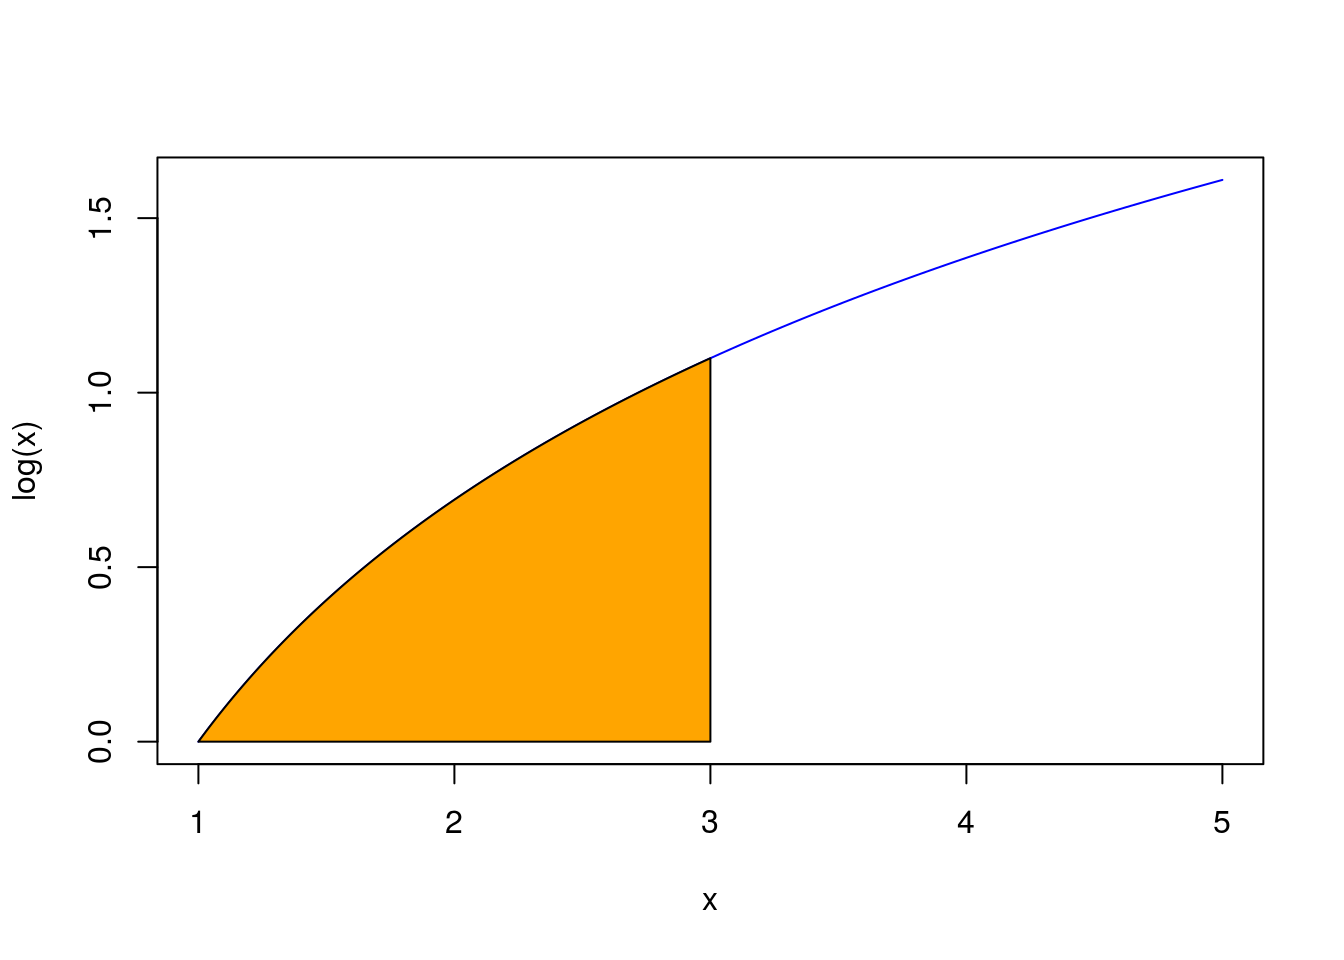
\includegraphics{Introduccion_prob_estad_bookdown_files/figure-latex/unnamed-chunk-12-1.pdf}

Hasta el momento hemos definidos las operaciones de división por
\(2\) y exponensialización por \(2\) las cuales fueron aplicadas
sobre \(10\). Esto es un ejemplo de un \emph{dominio de operaciones (PENSAR)}
sobre \(10\), es decir la lista

\[  10, \mbox{Op}_1, \mbox{Op}_2 \]

que comprende el objeto y las operaciones a ser aplicadas sobre.
El domino de operaciones nos habilita a trabajar con datos. Sumado
a \(\wedge\) y \(\hookrightarrow\) realizamos operaciones de forma
ordena (* arreglar).

Esta lista puede ser reproducible en el software \emph{R} (o en
\emph{Python} o \emph{C}\(++\)) definiendo \(\mbox{Op}_1(x)=\)\texttt{function(x)\ x/2} y \(\mbox{Op}_2(x)=\)\texttt{function(x)\ x\^{}2}. En la práctica, este
dominio de operaciones debe existir en la \emph{memoria temporal} de un
programa computacional. En este ejemplo con R, esto puede ser
ejecutado mediante los códigos

\begin{verbatim}
x = 10  # definimos que x será 10,
op1=function(x) x/2 # creamos Op1 ,  
Op2=function(x) x^2 # creamos Op2,
\end{verbatim}

los cuales quedarán guardados en nuestra memoria temporal de \emph{R}

\begin{definition}
\protect\hypertarget{def:unnamed-chunk-13}{}{\label{def:unnamed-chunk-13} }Un \textbf{dominio de operaciones} sobre objeto \(x\) es una lista de
operaciones que pueden ser aplicadas sobre \(x\) y el propio
elemento, es decir:
\[ x, \mbox{Op}_1, \ldots, \mbox{Op}_n. \]
\end{definition}

\hypertarget{operaciuxf3n-sobre-puntos}{%
\section*{Operación sobre puntos}\label{operaciuxf3n-sobre-puntos}}
\addcontentsline{toc}{section}{Operación sobre puntos}

Un tipo de operaciones que consideraremos en este trabajo es la de
representar un conjunto de puntos en el plano cartesiano o en el
espacio Euclineado tridimensionaL o un simple número.

\includegraphics{Introduccion_prob_estad_bookdown_files/figure-latex/unnamed-chunk-14-1.pdf}

\hypertarget{operaciuxf3n-cotideanas-sobre-puntos}{%
\subsection*{Operación cotideanas sobre puntos}\label{operaciuxf3n-cotideanas-sobre-puntos}}
\addcontentsline{toc}{subsection}{Operación cotideanas sobre puntos}

Destaco que funciones, como
la logaritmica \(\log: (0,\infty) \to \mathbb{R}\) es un
conjunto de puntos del tipo\\
\(\{(x,y)\in \mathbb{R}\times \mathbb{R}: y=\log(x) \mbox{ para } x\in (0,\infty) \} \subseteq \mathbb{R} \times \mathbb{R}\).

La función \(\log(x)\) puede ser representada en una hoja de
papel buscando sus puntos criticos y esbozando una dibujo. En
este documento estaremos interesados en gráficas generada
por programas computacionales. En el caso del programa \emph{R}
este puede ser representado por la operación \(Op_3(f)=\)
curve(f,from= x1, to= x2, col=``nombre color''), donde \(f\) es la
función de una variable que queremos graficar, x1 es valor
inicial, x2 el valor final sobre el cúal evaluaremos \(f\) y col es
el color de la curva.

En \emph{R} este es implementado por:

\begin{Shaded}
\begin{Highlighting}[]
   \KeywordTok{curve}\NormalTok{( }\KeywordTok{log}\NormalTok{(x), }\DataTypeTok{from =} \FloatTok{0.1}\NormalTok{, }\DataTypeTok{to =} \DecValTok{10}\NormalTok{ , }\DataTypeTok{col =} \StringTok{"green"}\NormalTok{, }\DataTypeTok{main =} \StringTok{"Gráfico función logarítmica"}\NormalTok{)}
\end{Highlighting}
\end{Shaded}

Lo cual produce la siguiente representación

\begin{center}\includegraphics{Introduccion_prob_estad_bookdown_files/figure-latex/unnamed-chunk-16-1} \end{center}

Ademas de gráficar \(\log(x)\), podemos trasnformar esta
función de una forma lineal en otra función que
simbolizaremos por \(\log^{*}\) la cual es dada por
\[ \mbox{Op}_4(\log(x)) = \log^{*}(x) = 2 + 5\log(x).\]

En \emph{R} esta transformación puede ser implementado por

\begin{Shaded}
\begin{Highlighting}[]
\NormalTok{  log}\OperatorTok{*}\StringTok{ }\ErrorTok{<}\OperatorTok{-}\StringTok{ }\ControlFlowTok{function}\NormalTok{(x) }\DecValTok{2} \OperatorTok{+}\StringTok{ }\DecValTok{5}\OperatorTok{*}\KeywordTok{log}\NormalTok{(x).}
\end{Highlighting}
\end{Shaded}

Otra operación que podemos realizar con \(\log\) es calcular el
área bajo la curva en el intervalo
\((1,3)\), es decir, la integral \[\int_{1}^{3} \log(x)dx\]
representado gráficamente

\begin{center}\includegraphics{Introduccion_prob_estad_bookdown_files/figure-latex/unnamed-chunk-18-1} \end{center}

La cual puede ser calculado via la operación
\(\mbox{Op}_5(f)\)=integrate(f, lower=, upper=), en que \(f\) es la
función a ser integrada, lower y upper son las cotas del
intervalo de integración.

\begin{Shaded}
\begin{Highlighting}[]
  \KeywordTok{integrate}\NormalTok{(log, }\DataTypeTok{lower=}\DecValTok{1}\NormalTok{, }\DataTypeTok{upper=}\DecValTok{3}\NormalTok{)}
\end{Highlighting}
\end{Shaded}

obteniendo el resultado

\begin{verbatim}

  1.295837 with absolute error < 1.4e-14,
  
\end{verbatim}

Es decir el área es aproximadamnete igual a \(1.29\) con un error
(absoluto) menor a \(1.4e-14\).

\begin{example}
\protect\hypertarget{exm:unnamed-chunk-20}{}{\label{exm:unnamed-chunk-20} }
En este caso, nuestro dominio de operaciones sobre el conjunto
\(\log(x)\) es la lista:

\[   \log(x), \mbox{Op}_3, \mbox{Op}_4.    \]
\end{example}

\hypertarget{operaciuxf3n-multivaria}{%
\section*{Operación multivaria}\label{operaciuxf3n-multivaria}}
\addcontentsline{toc}{section}{Operación multivaria}

Una operación artimetica en general es una operación multivariada
que transforma una lista ordenada de números \(x_1, \ldots, x_n\) en un
número \(x\), para \(n=1,2,...\).

\includegraphics{Introduccion_prob_estad_bookdown_files/figure-latex/unnamed-chunk-21-1.pdf}

La suma, el producto y la
exponencialización por dos puden ser
definidos de esta manera. Veamos los siguientes ejemplos

\begin{example}
\protect\hypertarget{exm:unnamed-chunk-22}{}{\label{exm:unnamed-chunk-22} }
La suma de \(n\) números naturales es una operación
\begin{eqnarray*}
\mbox{Op}_5: \mathbb{N} \times \ldots \times \mathbb{N} ( \mbox{n-veces})  \to \mathbb{N}\\
  (x_1,\ldots,x_n) \mapsto x_1 + \ldots + x_n. 
\end{eqnarray*}

La multiplicación de \(n\) números naturales es una operación\\
\begin{eqnarray*}
\mbox{Op}_6: \mathbb{N}\times \ldots \times \mathbb{N} ( \mbox{n-veces})  \to \mathbb{N}\\
  (x_1,\ldots,x_n) \mapsto x_1 \times \ldots \times x_n.
\end{eqnarray*}

Un ejemplo de exponensialización de \(n\) números naturales es una operación

\begin{eqnarray*}
\mbox{Op}_7: \mathbb{N}\times \ldots \times \mathbb{N} ( \mbox{n-veces})  \to \mathbb{N}\\
  (x_1,\ldots,x_n) \mapsto x_1^2 + \ldots + x_n^2.
\end{eqnarray*}
\end{example}

\begin{example}
\protect\hypertarget{exm:unnamed-chunk-23}{}{\label{exm:unnamed-chunk-23} }Otro ejemplo de operación es la composición:
\[ \mbox{Op}_7 \circ \mbox{Op}_5 (x_1,\ldots, x_n)= (x_1+\ldots
                                                       x_n)^2.\]
El dominio de aplicaciones
\[(x_1,\ldots, x_n), \mbox{Op}_5, \mbox{Op}_6, \mbox{Op}_7.\]
\end{example}

\hypertarget{operaciuxf3n-matricial}{%
\section*{Operación matricial}\label{operaciuxf3n-matricial}}
\addcontentsline{toc}{section}{Operación matricial}

Una operación matrices transforma una matriz en otra matriz, en un
vector o en un escalar.

\includegraphics{Introduccion_prob_estad_bookdown_files/figure-latex/unnamed-chunk-24-1.pdf}

\hypertarget{operaciuxf3n-probabilistica-o-estaduxedstica}{%
\section*{Operación probabilistica o estadística}\label{operaciuxf3n-probabilistica-o-estaduxedstica}}
\addcontentsline{toc}{section}{Operación probabilistica o estadística}

En este trabajo estaremos interesados en \textbf{operaciones
probabilisticas y estadísticas}, las cuales
transforman \textbf{eventos aleatorios} y \textbf{muestras de variables} en resumenes,
gráficos e inferencias. Mencionamos aquellas que serán
de nuestro interes.

\begin{enumerate}
\def\labelenumi{\arabic{enumi}.}
\tightlist
\item
  \textbf{Experimentar}: transformar una serie de pasos estipulados por
  la literatura científica en una observación empírica o
  subjetiva desde un objeto de estudio.
\end{enumerate}

\begin{example}
\protect\hypertarget{exm:unnamed-chunk-25}{}{\label{exm:unnamed-chunk-25} }
El curso de Elementos de Probabilidad e Inferencia Estadistica (EPIE) de este año tendrá dos secciones con un total
de 100 alumnos quienes aprobaron
el curso de Estadistica básica durante el semestre pasado.

El profesor EPIE quiere tener información previa de su curso con
respecto a su desempeño en el curso anterior. Para esto, ejecuta
un péqueño experimento: usa un generador de números aleatorio y
elige 30 de los 100 alumnos a los cuales les envia un correo
preguntando su carrera y promedio en el curso anterior.

El profesor obtiene una muestra \(x=(x_1,\ldots,x_{30})\) de
promedios y la lista \(c=(c_1,\ldots, c_{30})\) de sus
correspondientes carreras encontrando: ingenieria cívil industrial, ingenieria química e
ingeniería en recursos naturales.
\end{example}

\begin{enumerate}
\def\labelenumi{\arabic{enumi}.}
\setcounter{enumi}{1}
\tightlist
\item
  \textbf{Cuantificar} y \textbf{categorizar}: codificar una observación por un
  número o una categoría (clasificación conceptual).
\end{enumerate}

\begin{example}
\protect\hypertarget{exm:unnamed-chunk-26}{}{\label{exm:unnamed-chunk-26} }
Podemos contar el número de repeticiones de cada carrera, por ejemplo: ingenieria cívil industrial (8), ingenieria
química (11) e ingeniería en recursos naturales (11).

También podemos categorizar cada promedio según sea mayor o menor a 5.8, obteniendo la transformación de los promedios
\(y=(y_1,\ldots,y_{30})\) en que \(y_i=1\) si \(x_i\leq 5.8\) y \(y_i=0\) en el caso contrario.
\end{example}

\begin{enumerate}
\def\labelenumi{\arabic{enumi}.}
\setcounter{enumi}{2}
\tightlist
\item
  \textbf{Reducir}: transformar un objeto en otro menor dimensión y
  complejidad.
\end{enumerate}

\begin{example}
\protect\hypertarget{exm:unnamed-chunk-27}{}{\label{exm:unnamed-chunk-27} }Podemos reducir la muestra de los promedios al promedio de los promedios
\((x_1,\ldots,x_{30}) \mapsto \frac{1}{30}(x_1+\ldots+x_{30})\) obteniendo \(\bar{x}= 5 .5\).

Podemos reducir las categorias \(y\) a la proporción de notas mayores y menores a \(5 .8\)
\((y_1,\ldots,y_{30}) \mapsto (p1,p2)\), en que \(p1= 45\%\)
y \(p2= 55\%\), mayor o menor, respectivamente.
\end{example}

\begin{enumerate}
\def\labelenumi{\arabic{enumi}.}
\setcounter{enumi}{3}
\tightlist
\item
  \textbf{Gráficar}: transformar una lista de puntos en un objeto visual.
\end{enumerate}

\begin{example}
\protect\hypertarget{exm:unnamed-chunk-28}{}{\label{exm:unnamed-chunk-28} }
Para la muestra de promedio \(x\) podemos representarlos en un gráfico de caja y bigotes. Para las categorías
\(y\) un gráfico de barras.
\end{example}

\includegraphics{Introduccion_prob_estad_bookdown_files/figure-latex/unnamed-chunk-30-1.pdf}

\begin{enumerate}
\def\labelenumi{\arabic{enumi}.}
\setcounter{enumi}{4}
\tightlist
\item
  \textbf{Describir}: transformar una observación y/o cuantificación y/o categorización en una caracteristica
  de un objeto sin pretender deducir o inducir.
\end{enumerate}

\begin{example}
\protect\hypertarget{exm:unnamed-chunk-31}{}{\label{exm:unnamed-chunk-31} }
El centroide de los promedios observados es igual a 5.5, es decir, la muestra de promedios gravita entorno al centro 5.5. Los promedios más frecuente son menores a 5.8.
\end{example}

\begin{enumerate}
\def\labelenumi{\arabic{enumi}.}
\setcounter{enumi}{5}
\tightlist
\item
  \textbf{Estimar}: cuantificar o categorizar un fenomeno desconocido con base a la observación
  parcial acerca de él desde un experimento.
\end{enumerate}

\begin{example}
\protect\hypertarget{exm:unnamed-chunk-32}{}{\label{exm:unnamed-chunk-32} }
En base a la muestra, estimo que el promedio de notas del curso Estadística es aproximadamente 5.5.
En base a la muestra, la proporción de promedios menores a 5.8 es igual a a 55\%.
\end{example}

\begin{enumerate}
\def\labelenumi{\arabic{enumi}.}
\setcounter{enumi}{6}
\tightlist
\item
  \textbf{Inferir}: deducir o inducir conclusiones sobre un fenomeno desconocido con base a la observación
  parcial acerca de él desde un experimento.
\end{enumerate}

\begin{example}
\protect\hypertarget{exm:unnamed-chunk-33}{}{\label{exm:unnamed-chunk-33} }
En base a la muestra, estimo que el promedio de notas del curso Estadística es aproximadamente 5.5.
En base a la muestra, la proporción de promedios menores a 5.8 es igual a a 55\%.
\end{example}

\begin{enumerate}
\def\labelenumi{\arabic{enumi}.}
\setcounter{enumi}{7}
\tightlist
\item
  Componer: elaborar un objeto tomando partes o propiedades de otros.
\end{enumerate}

\begin{example}
\protect\hypertarget{exm:unnamed-chunk-34}{}{\label{exm:unnamed-chunk-34} }
Pensar.
\end{example}

\hypertarget{operaciuxf3n-funciuxf3n-matemuxe1tica}{%
\section*{\texorpdfstring{Operación \(=\) función matemática}{Operación = función matemática}}\label{operaciuxf3n-funciuxf3n-matemuxe1tica}}
\addcontentsline{toc}{section}{Operación \(=\) función matemática}

La propiedad de una operación Op se estudia al escribirla como
una función:\\
\[  \begin{aligned}
  \mbox{Op}: \mbox{Dom} \to \mbox{Rec}, & \\
  A \mapsto \mbox{Op}(A),&
  \end{aligned}
  \] en donde Dom y Rec son el dominio y recorrido de Op,
respectivamente. En términos simples, Dom es la lista de los
objetos sobre los cuales actua Op y Rec es la lista de las
transformaciones que Op puede realizar.

Ambas operaciones pueden ser formalizadas como funciones
consideremos el dominio y recorrido
\(\mbox{Dom}=\mbox{Rec}=\mathbb{N}\). Por ejemplo:

\[  \begin{aligned}
  \mbox{Op}_1: \mathbb{N} \to \mathbb{N}, & \\
  x \mapsto \mbox{Op}_1(x)= x/2,&
  \end{aligned} \]

Formalmente, dado que \(\mbox{Op}_1\) y \(\mbox{Op}_2\) son funciones,
formalmente, la aplicación secuencial de estas operaciones sobre
\(A\) es la composición de funciones\\
\[
  \begin{aligned}
  \mbox{Op}_2 \circ \mbox{Op}_1: \mbox{Dom}_1 \to \mbox{Rec}_1=\mbox{Dom}_2
  \to \mbox{Rec}& \\
  A \mapsto    \mbox{Op}_2\left( 
    \mbox{Op}_1(A) \right).&
  \end{aligned}
  \]

\hypertarget{organizaciuxf3n-del-documento}{%
\section*{Organización del documento}\label{organizaciuxf3n-del-documento}}
\addcontentsline{toc}{section}{Organización del documento}

El Capitulo \(1\) presenta los elementos básicos de análisis
exploratorio y resumen de datos uni y bivariado.

\hypertarget{datos}{%
\chapter{Reducir y gráficar}\label{datos}}

\hypertarget{conceptos-elementales}{%
\section{Conceptos elementales}\label{conceptos-elementales}}

En esta sección presento conceptos básicos para
este
curso.

\begin{definition}
\protect\hypertarget{def:unnamed-chunk-37}{}{\label{def:unnamed-chunk-37} }(a) Una \textbf{población} es un conjunto de personas,
objetos
o eventos, de los
cuales nos interesa estudiar algunas de sus
características. (b) \textbf{Medidas poblacionales} son
listas
de mediciones de ciertas cantidades provenientes
de cada
individuo o elemento de la población. (c) Un
\textbf{parámetro
poblacional} es una característica general de la
población.
\end{definition}

Presento tres ejemplos de población, unidades
poblacionales y parámetros poblacionales.

\begin{example}
\protect\hypertarget{exm:unnamed-chunk-38}{}{\label{exm:unnamed-chunk-38} }(a) \emph{Población}: total de autos cuyos modelos
salieron a
la venta en un determinado intervalo de tiempo y
funcionan en una determinada país. (b) \emph{Medidas
poblacionales}: razón de millas recorrida por
galón de
combustible, número de cilindro, caballos de
fuerza, tipo
de caja de cambios. (c) \emph{Parámetro poblacional}:
media
poblacional de razón de millas recorrida por galón
de
combustible, media poblacional de caballos de
fuerza y
proporción de autos con caja de cambio automático.
\end{example}

\begin{example}
\protect\hypertarget{exm:unnamed-chunk-39}{}{\label{exm:unnamed-chunk-39} }(a) \emph{Población}: individuos de una cierta comuna
de una
ciudad que poseen problemas de insulina.
(b) \emph{Medidas poblacionales}: presencia o no de
menarquía
(primera hemorragia menstrual de la mujer), edad,
sexo,
nivel de igf1 (factor de crecimiento insulínico
tipo 1,),
etapa de la pubertad y nivel testicular. (c)
\emph{Parámetro
poblacional}: promedio de edad poblacional,
frecuencias
relativas de etapas de la pubertad poblacional y
media
poblacional de igf\(1\).
\end{example}

\begin{example}
\protect\hypertarget{exm:unnamed-chunk-40}{}{\label{exm:unnamed-chunk-40} }(a) \emph{Población}: pacientes de una determinada
comunidad
que reciben tres métodos diferentes de
ventilación durante la anestesia. (b) \emph{Medidas
poblacionales}: concentración de folato
(microgramos por litro) y tipo de ventilación
recibida
por los pacientes\footnote{(i) \$\mbox{N$2$O} +
  \mbox{O}2\$, \(24\)h: \(50\%\) de óxido nitroso y
  \(50\%\) de
  oxígeno, de forma continua durante \(24\)
  horas; (ii) N2O + O2, op: \(50\%\) de óxido nitroso
  y
  \(50\%\) de oxígeno, solo durante el
  funcionamiento; (iii) \(O2.24h\): sin óxido nitroso
  pero
  entre un \(35\%\) y un \(50\%\) de oxígeno
  durante \(24\) horas}. \emph{Parámetros poblacionales}:
media
de folato poblacional y proporciones de
factores de niveles de ventilación.
\end{example}

Los conceptos de unidad de observación (o
muestral),
muestra y base de datos son presentados a
continuación.

\begin{definition}
\protect\hypertarget{def:unnamed-chunk-41}{}{\label{def:unnamed-chunk-41} }(a) \textbf{Unidades de observaciones:} es un grupo de
elementos de una población de la cual es
posible obtener mediciones.
Comunmente es conocido como una \textbf{muestra} de la población.
(b) Un \textbf{experimento} es una operación bien
planificada y controlada que se realiza para
obtener las mediciones desde algunas unidades de
observación de una determinada población. (c) Las
mediciones cuantificada o codificada derivada de
un experimento es llamada de \textbf{datos}. (d)
Una \textbf{base de datos} es una forma ordenada
organizados la muestra de tal manera de que estos
puedan
ser trabajados por programas
computacionales.
\end{definition}

\textbf{Nota}: en general, el experimento debe ser
realizado
por un procedimiento que evite el sesgo
personal. Esto podría lograrse utilizando algún
\emph{mecanismo aleatorio}. Sin embargo, esto no
siempre es posible debido a problemas ético y
legales.
Esto ocurre en el caso de estudios en el
área de la salud donde aplicar un mecanismo
aleatorio
podría poner en peligro la integridad de los
pacientes. En este caso, el experimento se reduce un
estudio de los datos disponibles.

Presentamos algunos ejemplos.

\begin{example}
\protect\hypertarget{exm:unnamed-chunk-42}{}{\label{exm:unnamed-chunk-42} }(a) \emph{Unidad de observación}: grupo de autos de una
determinada ciudad. (b) \emph{Experimento}: escoger
autos de forma aleatoria de una determinada ciudad y
medir razón de millas recorrida por galón de
combustible, número de cilindro, caballos de fuerza, tipo
de caja de cambios. (c) \emph{Muestra}: lista de estos valores
observados en la medición. (d) \emph{Base de datos}: vector
columna con los datos de
una característica observada o matriz rectangular con
toda la información codificada.
\end{example}

Mostraremos un ejemplo de datos en forma de vector y
matriz con la base de datos \emph{mtcars} del
paquete de \emph{R} llamado \emph{MASS}. Esta base de datos está en
formato de \emph{data frame} y fue publicado
en \(1974\) en la revista \emph{Motor Trend US magazine}. La
base \emph{mtcars} contiene datos de \(32\) autos
de modelos diferentes. Por ejemplo, la razón de millas
por galón de combustible (mpg) en forma de
vector columna de los primeros y últimos valores

\[\mbox{mpg}=(21.0 ; 21.0 ; 22.8 ; 21.4 ,\ldots, 27.3 ;
26.0 ; 30.4 ; 15.8 ; 19.7 ; 15.0 ;
21.4)^\top. \]

En la siguiente matriz se presenta en la primera columna
el modelo de los autos estudiados y en
las restantes columnas las variables medidas para los \(6\)
primeros autos estudiados. Aquí, por
ejemplo, ``Mazda RX4'' es el modelo del primer auto, cuya
\emph{mpg} o razón de millas por galón es
igual a \(21\) y su \emph{cyl} o número de cilindros del motor
es igual a \(6\).

\begin{verbatim}
##                    mpg cyl disp  hp drat    wt  qsec vs am gear carb
## Mazda RX4         21.0   6  160 110 3.90 2.620 16.46  0  1    4    4
## Mazda RX4 Wag     21.0   6  160 110 3.90 2.875 17.02  0  1    4    4
## Datsun 710        22.8   4  108  93 3.85 2.320 18.61  1  1    4    1
## Hornet 4 Drive    21.4   6  258 110 3.08 3.215 19.44  1  0    3    1
## Hornet Sportabout 18.7   8  360 175 3.15 3.440 17.02  0  0    3    2
## Valiant           18.1   6  225 105 2.76 3.460 20.22  1  0    3    1
\end{verbatim}

Te presento un ejemplo en el area de la salud.

\begin{example}
\protect\hypertarget{exm:unnamed-chunk-44}{}{\label{exm:unnamed-chunk-44} }(a) \emph{Unidad de observación}: pacientes de un determinado
hospital. (b) \emph{Experimento}: examen de
laboratorio en donde se escogen individuos para medir:
presencia o no de menarquía (primera
hemorragia menstrual de la mujer), edad, sexo, nivel de
igf\(1\) (factor de crecimiento insulínico
tipo \(1\),), etapa de la pubertad y nivel testicular. (c)
\emph{Muestra}: mediciones de estos valores.
(d) \emph{Base de datos}: vector columna con los datos de una
característica observada o matriz
rectangular con toda la información codificada.
\end{example}

La siguiente base de datos llamada \emph{juul2} proviene dal
paquete \emph{ISwR} del programa R. Contiene
información de pacientes con problema de insulina. Aquín,
por ejemplo, \emph{age} contiene la edad de
los pacientes y \emph{menarche} presencia o no de menarquía
(primera hemorragia menstrual de la
mujer).

\begin{verbatim}
##     age height menarche sex igf1 tanner testvol weight
## 1    NA     NA       NA  NA   90     NA      NA     NA
## 2    NA     NA       NA  NA   88     NA      NA     NA
## 3    NA     NA       NA  NA  164     NA      NA     NA
## 4    NA     NA       NA  NA  166     NA      NA     NA
## 5    NA     NA       NA  NA  131     NA      NA     NA
## 6  0.17     NA       NA   1  101      1      NA     NA
## 7  0.17     NA       NA   1   97      1      NA     NA
## 8  0.17     NA       NA   1  106      1      NA     NA
## 9  0.17     NA       NA   1  111      1      NA     NA
## 10 0.17     NA       NA   1   79      1      NA     NA
## 11 0.17     NA       NA   1   43      1      NA     NA
## 12 0.17     NA       NA   1   64      1      NA     NA
## 13 0.25     NA       NA   1   90      1      NA     NA
## 14 0.25     NA       NA   1  141      1      NA     NA
## 15 0.42     NA       NA   1   42      1      NA     NA
\end{verbatim}

Es normal que al aplicar la medición ocurran errores o
problemas con los instrumentos de medición.
Las normas éticas científicas exigen no ocultar esto sino
informarlas. Por ejemplo,
un símbolo \textbf{NA} indica que el valor fue perdido. El
símbolo \textbf{NULL} indica que el valor
obtenido fue nulo o no tiene validez. Se simboliza por
\textbf{Inf} para valores que salieron fuera de
los límites de los valores de medición del instrumento.

Presentamos otro ejemplo dentro del área de la salud.

\begin{example}
\protect\hypertarget{exm:unnamed-chunk-47}{}{\label{exm:unnamed-chunk-47} }\emph{Unidad de observación}: pacientes de un determinado
hospital. \emph{Experimento}: examen de
laboratorio en donde se reciben pacientes y se les mide
concentración de folato (microgramos por
litro) y factores con niveles de N2O+O2. \emph{Muestra}:
lista de estos valores. \emph{Base de datos}:
vector o matriz rectangular con estos datos
cuantificados.\\
\end{example}

\begin{verbatim}
##    folate ventilation
## 1     243  N2O+O2,24h
## 2     251  N2O+O2,24h
## 3     275  N2O+O2,24h
## 4     291  N2O+O2,24h
## 5     347  N2O+O2,24h
## 6     354  N2O+O2,24h
## 7     380  N2O+O2,24h
## 8     392  N2O+O2,24h
## 9     206   N2O+O2,op
## 10    210   N2O+O2,op
\end{verbatim}

Podemos resumir el proceso de análisis de datos en la
siguiente figura

Todo comienza con el interés por conocer atributos
desconocidos de una determinada población. Aquí
son llamados de parámetros poblacionales. Para \emph{aprender}
de estos parámetros se realiza un
experimento y recopilar información. El siguiente paso es
\emph{explorar} las características generales
de los datos. Luego buscaremos resumirlos para sacar
conclusiones preliminares sobre los
parámetros poblacionales.

\hypertarget{variables-observadas-en-experimentos}{%
\section{Variables observadas en experimentos}\label{variables-observadas-en-experimentos}}

Un elemento relevante de la planificación de un
experimento científico es el conjunto de variables que
será medido desde las unidades de observación.

\begin{definition}
\protect\hypertarget{def:unnamed-chunk-50}{}{\label{def:unnamed-chunk-50} }(a) Una \textbf{variable} \(X\) es una característica de interés
que posee cada elemento de una población
y que podemos medir. (b) Una variable es \textbf{cuantitativa}
si sus valores son números y representan
una cantidad. (c) Una variable es \textbf{cualitativa} si sus
valores representan una cualidad, un
atributo o una categoría. Se les llama también variables
categóricas. (d) Una lista

\[x_1, x_2, \ldots, x_n\]
de observaciones de una variable \(X\) obtenidas al
desarrollar un experimento es llamada de
\textbf{datos observados} de \(X\) extraída desde una lista
de \(n\) unidades de observación. El número \(n\)
será llamado de \textbf{tamaño de los datos}.
\end{definition}

Presentamos algunos ejemplos.

\begin{example}
\protect\hypertarget{exm:unnamed-chunk-51}{}{\label{exm:unnamed-chunk-51} }- Ejemplo de variables cuantitativas:

\begin{verbatim}
    - Razón de millas por galón de combustible. 
    - Número de cilindros  de motores.
    - Número de caballos de fuerza de motores.
    - Peso en Kilogramos.
    - Nivel de insulina en la sangre.
    - Temperatura en grados Celsius (o Fahrenheit).
    - Año de lanzamiento de un modelo de auto.
\end{verbatim}
\end{example}

\begin{example}
\protect\hypertarget{exm:unnamed-chunk-52}{}{\label{exm:unnamed-chunk-52} }Ejemplo de variables cualitativas:

\begin{verbatim}
- Tipo de motor.
- Modelo del auto.
- Sexo.
- Tipo de ventilación en pacientes.  
\end{verbatim}
\end{example}

En general, las variables de experimentos son
clasificadas en dos tipo.

\begin{definition}
\protect\hypertarget{def:unnamed-chunk-53}{}{\label{def:unnamed-chunk-53} }
Tipos de variables cuantitativas. (a) \textbf{Discreta:} si
el conjunto de todos sus posibles valores
tiene un número finito de elementos, o bien es infinito,
pero se pueden numerar uno por uno de acuerdo al conjunto
de número naturales
\(\{0,1,2,3,\ldots\}\). Noten que, esto implica que la
variable puede asumir solamente un conjunto
finito de valores dentro de un intervalo \((a,b)\). Una
variable discreta puede asumir valores con
decimales. (b) \textbf{Continua:} si puede tomar todos los
valores posibles dentro de un intervalo de
números reales, como por ejemplo \((a,b)\) o \([a,b]\).
\end{definition}

Presentamos algunos ejemplos.

\begin{example}
\protect\hypertarget{exm:unnamed-chunk-54}{}{\label{exm:unnamed-chunk-54} }Ejemplo de variables discretas:

\begin{verbatim}
- Número de cilindros  de motores.
- Número de caballos de fuerza de motores.
- Una variable hipotética con valores: 0, 0.5, 1, 1.5, 2, 2.5, ...
\end{verbatim}

.
\end{example}

\begin{example}
\protect\hypertarget{exm:unnamed-chunk-55}{}{\label{exm:unnamed-chunk-55} }Ejemplo de variables continuas:

\begin{verbatim}
- Razón de millas por galón de combustible. 
- Peso en Kilogramos.
- Nivel de insulina en la sangre.
- Temperatura en grados Celsius (o Fahrenheit).
\end{verbatim}
\end{example}

Luego de obtener los resultados de un experimento, el
investigador debe codificar los resultados para poder
construir la base de datos. En el caso de variables
cualitativas, esto es hecho clasificándola en dos tipos
de escala de medición.

\begin{definition}
\protect\hypertarget{def:unnamed-chunk-56}{}{\label{def:unnamed-chunk-56} }Escalas de mediciones de variables cualitativas. (a)
\textbf{Escala nominal:} si sus valores son
etiquetas o atributos y no existe un orden jerárquico
entre ellos. (b) \textbf{Escala ordinal:} si sus
valores son etiquetas o atributos pero existe un cierto
orden jerárquico entre ellos.
\end{definition}

\begin{example}
\protect\hypertarget{exm:unnamed-chunk-57}{}{\label{exm:unnamed-chunk-57} }Ejemplo de variables cualitativas en escala nominal:

\begin{verbatim}
- Tipo de motor.
- Sexo.
- Tipo de ventilación en pacientes.  
- Idioma.
- Nacionalidad.
\end{verbatim}
\end{example}

\begin{example}
\protect\hypertarget{exm:unnamed-chunk-58}{}{\label{exm:unnamed-chunk-58} }Ejemplo de variables cualitativas ordinal:

\begin{verbatim}
- Grupo etario: lactante, niños, adolescente, adulto
y tercera edad.
- Clasificación de productos tecnológicos: básico,
gama media y gamma alta. 
- Posición de llegada en una competencia.
- Talla de ropa: S, M, L, etc. 
- Tipo de ventilación en pacientes.   
\end{verbatim}
\end{example}

Las variables cuantitativas también son clasificadas
según su escala de medición.

\begin{definition}
\protect\hypertarget{def:unnamed-chunk-59}{}{\label{def:unnamed-chunk-59} }\textbf{Escala de intervalo:} existe una noción de distancia
entre los valores de la variable y no
existe necesariamente el valor natural cero como
indicador de ausencia de algo. En este caso el
cero u otro valor representa un punto de cambio de
``nivel''. En general, la escala una variable en
escala de intervalo es establecido vía consensos
científicos o de instituciones para estandarizar
procesos.
\end{definition}

\begin{definition}
\protect\hypertarget{def:unnamed-chunk-60}{}{\label{def:unnamed-chunk-60} }\textbf{Escala de razón} si los valores de la variable tienen
un sentido físico de \emph{intensidad} y
existe el cero indicando ausencia de valor. En este caso
el cero es el origen de los valores a ser
medidos.\\
\end{definition}

\begin{example}
\protect\hypertarget{exm:unnamed-chunk-61}{}{\label{exm:unnamed-chunk-61} }Ejemplo de variables cuantitativas medidas en escala de
intervalo:

\begin{verbatim}
- Escala de notas: de 0 a 7, de 0 a 10,
utilizando letras con números. 
- Puntaje PSU.
- El pH,  una medida de acidez o alcalinidad de 
una sustancia.
- Temperatura en grados Celsius (o Fahrenheit):
puede asumir valores positivos, negativos
y en particular ser igual a 0.
\end{verbatim}
\end{example}

\begin{example}
\protect\hypertarget{exm:unnamed-chunk-62}{}{\label{exm:unnamed-chunk-62} }Ejemplo de variables cuantitativas medidos en escala de
razón:

\begin{verbatim}
    - Razón de millas por galón de combustible. 
    - Número de cilindros  de motores.
    - Número de caballos de fuerza de motores.
    - Peso en Kilogramos.
    - Nivel de insulina en la sangre.
\end{verbatim}
\end{example}

\hypertarget{agrupamiento-de-variables}{%
\section{Agrupamiento de variables}\label{agrupamiento-de-variables}}

\begin{definition}
\protect\hypertarget{def:unnamed-chunk-63}{}{\label{def:unnamed-chunk-63} }(a) Una \textbf{clase} es un agrupamiento de \emph{categorías} en
el caso de variables cualitativas, o de
\emph{intervalos numéricos} en el caso de variables
cuantitativas. (b) Una \textbf{marca de clase} es un
dato que representa a una clase. En el caso de los
intervalos la marcha de clase es el punto medio
de los intervalos que se obtiene con el promedio de los
extremos.
\end{definition}

\begin{example}
\protect\hypertarget{exm:unnamed-chunk-64}{}{\label{exm:unnamed-chunk-64} }Consideremos los valores de las variables \emph{mpg} de la
base de datos \emph{mtcars}. Clasificando los
valores en intervalos de largo \(4.4\) mil millas por galón
obtenemos los intervalos

\[ [0 ; 4.4), [4.4 ; 8.8), [8.8 ; 13.2) [13.2 ; 17.6),
[17.6 ; 22.0), [22.0 ; 26.4), [26.4 ; 30.08] \]

La marca de clase para el intervalo \([13.2 ; 17.6)\) es
el punto \(15.4\). Analogamente para los
otros casos.
\end{example}

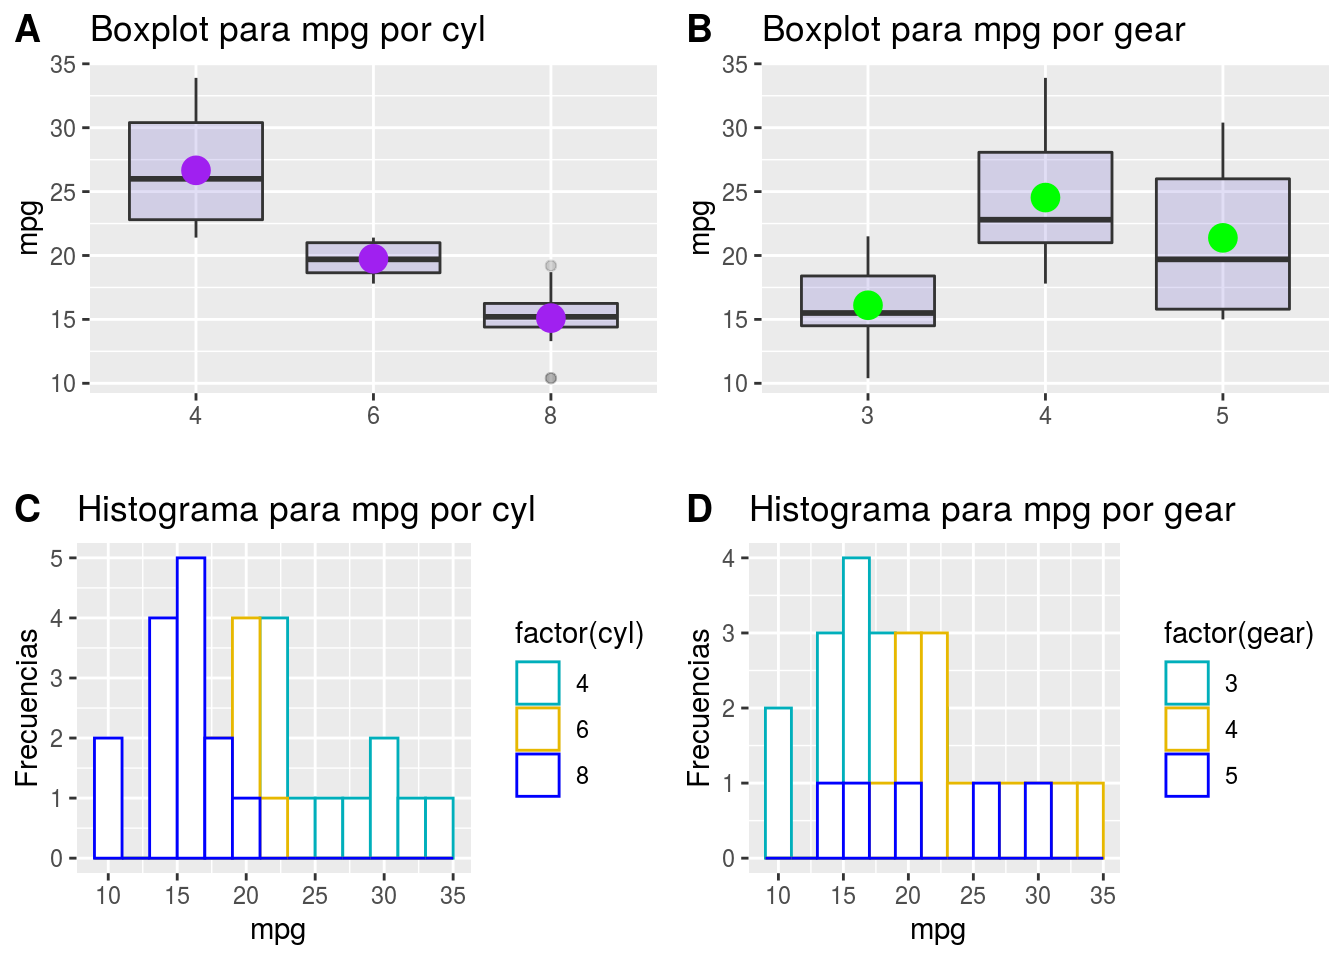
\includegraphics{Introduccion_prob_estad_bookdown_files/figure-latex/unnamed-chunk-65-1.pdf}

\hypertarget{operaciuxf3n-de-anuxe1lisis-exploratorio-de-datos}{%
\section{Operación de análisis exploratorio de datos}\label{operaciuxf3n-de-anuxe1lisis-exploratorio-de-datos}}

Antes de comenzar esta sección introduciendo una definición auxiliar. No es un concepto formal propiamente definida en la teoría, pero no servira para comunicarnos.

\begin{definition}
\protect\hypertarget{def:unnamed-chunk-66}{}{\label{def:unnamed-chunk-66} }
Llamaremos de \textbf{información estadísica} a transformaciones de los datos en
brutos a \emph{estructuras bien organizadas} nos ayudan a interpretar y obtener
informaciones de forma más clara. Por estructuras organizadas entenderemos
simplemente elementos organizados por una relación binarias y represetadas de
manera simplificada.
\end{definition}

\begin{definition}
\protect\hypertarget{def:unnamed-chunk-67}{}{\label{def:unnamed-chunk-67} }
La \textbf{estadística descriptiva} es la área de la
\textbf{Estadística} que se preocupada de la
aplicación de operaciones que transformen
los datos en información estadística.
\end{definition}

\begin{definition}
\protect\hypertarget{def:unnamed-chunk-68}{}{\label{def:unnamed-chunk-68} }La parte de la Estadística Descriptiva que utiliza
herramientas para \textbf{visualizar}
caracteristicas generales de los datos es llamada de
``Analisis exploratorio de Datos''. Tales
herramientas son llamadas de \textbf{operaciones
exploratorias}.
\end{definition}

\begin{example}
\protect\hypertarget{exm:unnamed-chunk-69}{}{\label{exm:unnamed-chunk-69} }Ejemplo de operaciones exploratoias son construir: tablas
de frecuencias, graficos de tallos y
hojas, histogramas, diagrama de caja y bigotes, diagrama
de dispersión, etc.
\end{example}

\hypertarget{operaciones-de-exploraciuxf3n-grafica-de-los-datos-sin-grupos}{%
\subsection{Operaciones de exploración grafica de los datos: sin grupos}\label{operaciones-de-exploraciuxf3n-grafica-de-los-datos-sin-grupos}}

Los gráficos estadísticos nos entregarán información
representada en el plano cartesiano bi o
tridimensional de los valores de la variable \(X\) que
acumula las mayores frecuencia y como se
distribuyen los otros datos en torno de estos valores
centrales, entre otros.

\begin{definition}
\protect\hypertarget{def:unnamed-chunk-70}{}{\label{def:unnamed-chunk-70} }
\textbf{Gráfico de tallos y hojas:} su aspecto es muy similar al de un
histograma dibujado horizontalmente. A los dígitos del primer
decimal de los números que aparecen listados en la parte
\emph{derecha} de \(|\) del diagrama se les llama \textbf{hojas} y a la parte
izquierda de la parte no decimal se le llama \textbf{tallo}.
\end{definition}

\begin{definition}
\protect\hypertarget{def:unnamed-chunk-71}{}{\label{def:unnamed-chunk-71} }\textbf{Gráfico circular o de torta:} para variables cualitativas o
bien para
variables cuantitativas agrupadas,
se pueden elaborar gráficas de pastel, también llamadas
pie charts. Estas son gráficas circulares divididas en sectores
que permiten comparar visualmente
las frecuencias porcentuales de los valores observados de
una variable.
\end{definition}

\begin{definition}
\protect\hypertarget{def:unnamed-chunk-72}{}{\label{def:unnamed-chunk-72} }
\textbf{Gráfico de barras:} las gráficas de barra ayudan a visualizar
los valores de una variable que
ocurren con mayor o menor frecuencia y a comparar
cualitativamente estas
frecuencias.
\end{definition}

\begin{definition}
\protect\hypertarget{def:unnamed-chunk-73}{}{\label{def:unnamed-chunk-73} }\textbf{Histograma::} un histograma es una gráfica muy similar a una
gráfica de barras. Adquiere este nombre cuando existe un orden
entre los valores de la variable a graficar. Nuevamente, para cada
valor, categoría o clase de la variable, se asocia una barra
cuya altura es la frecuencia con la que se observa la
categoría.
\end{definition}

\begin{definition}
\protect\hypertarget{def:unnamed-chunk-74}{}{\label{def:unnamed-chunk-74} }\textbf{Boxplot:} para representar los datos con base en valores que
dividan los datos en partes estratégicas es
adecuado usar un gráfico de tallos y hojas. Para su
diseño es necesario el valor mínimo, el primer
(C1), segundo (C2), tercer cuartil (C3) y el máximo de
los datos. La caja es formada por C1 y C3
en cuyo centro se encuentra C2 (la mediana.)
\end{definition}

Presento algunos ejemplos de transformaciones de los datos mpg en
gráficos.

\begin{verbatim}
## 
##   The decimal point is at the |
## 
##   10 | 44
##   12 | 3
##   14 | 3702258
##   16 | 438
##   18 | 17227
##   20 | 00445
##   22 | 88
##   24 | 4
##   26 | 03
##   28 | 
##   30 | 44
##   32 | 49
\end{verbatim}

\textbf{Interpretación:} el valor más frecuente de los valores observados
de \emph{mpg} son las medidas cuya parte entera es \(14\). En menor cantidad,
pero también frecuentes son los valores con parte entera igual a \(18\)
y \(20\).

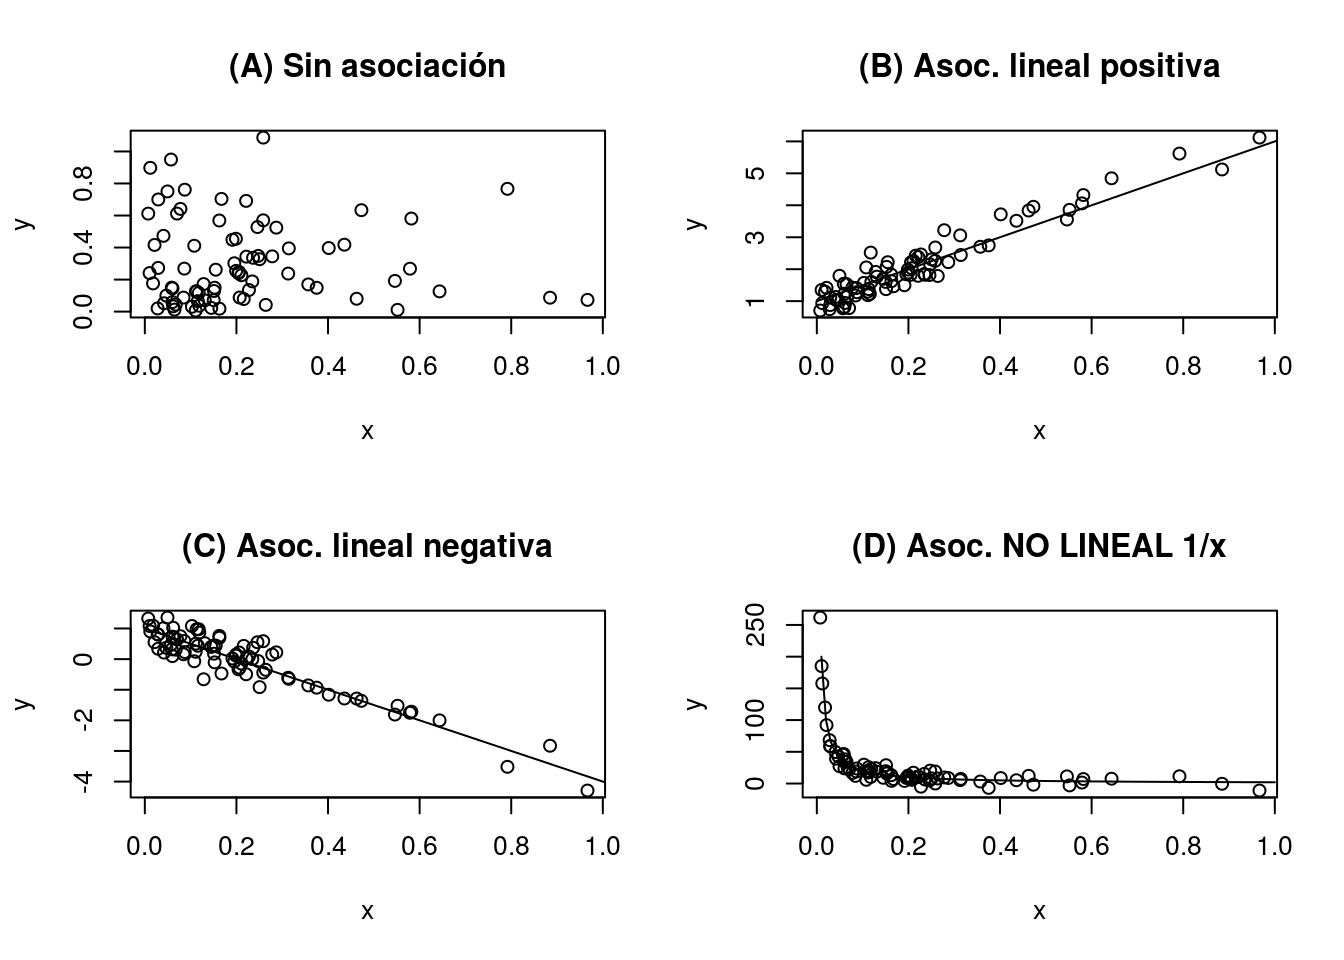
\includegraphics{Introduccion_prob_estad_bookdown_files/figure-latex/unnamed-chunk-76-1.pdf}

\textbf{Interpretación:} dentro de la base de datos mtcars, los autos con
\(8\) y \(4\) ciclos son los más frecuentes.

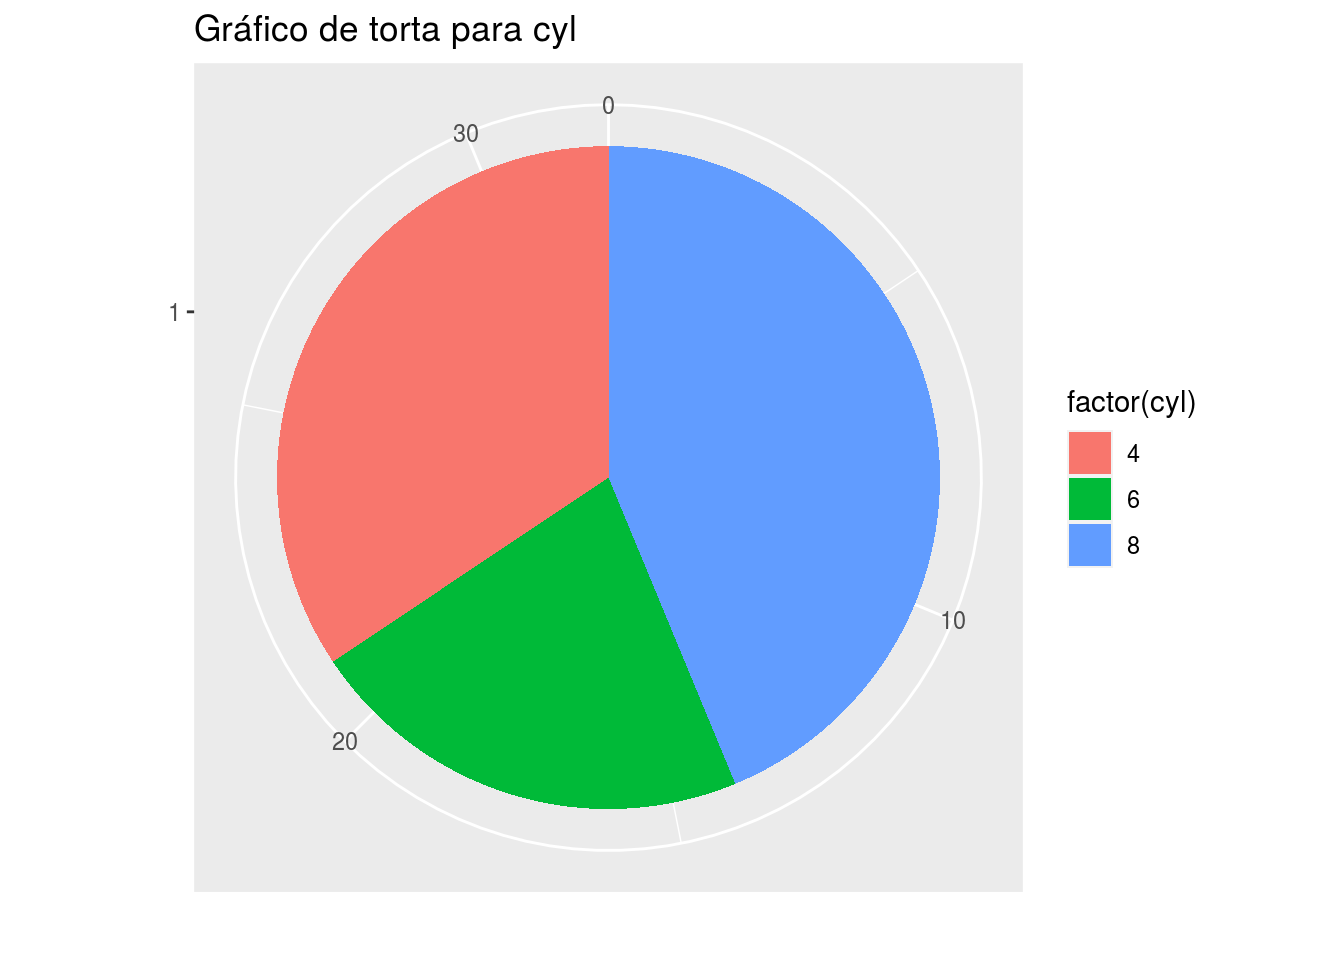
\includegraphics{Introduccion_prob_estad_bookdown_files/figure-latex/unnamed-chunk-77-1.pdf}

\textbf{Interpretación:} en la base de datos \emph{mtcars} los autos con cambio
de velocidad automático (\(0\)) es mayor que los autos con cambios
manual (\(1\)). Los autos cambio de velocidad automático suman un mayor
número de cilindros que los autos con cambios manuales. Las altas
frecuencias de mpg se concentran en torno a \(20\) millas por galón.

\hypertarget{operaciones-de-exploraciuxf3n-gruxe1fica-de-los-datos-por-grupos}{%
\subsection{Operaciones de exploración gráfica de los datos: por grupos}\label{operaciones-de-exploraciuxf3n-gruxe1fica-de-los-datos-por-grupos}}

Los gráficos por grupos nos ayudarán a comparar las
características de los datos separados por unidades
muestrales con alguna característica en común.

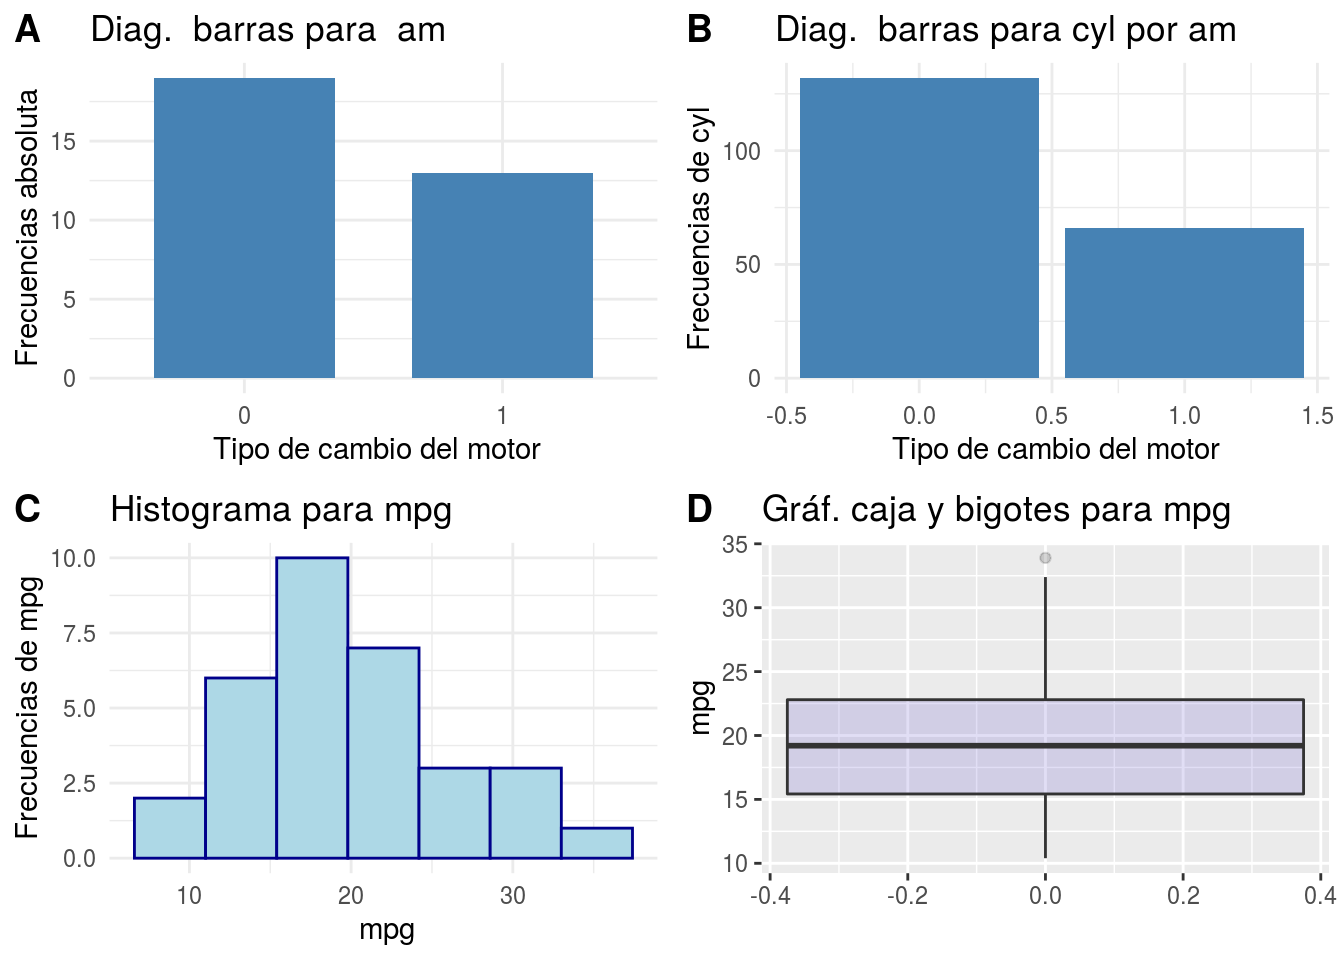
\includegraphics{Introduccion_prob_estad_bookdown_files/figure-latex/unnamed-chunk-78-1.pdf}
\textbf{Interpretación}: Los autos con \(4\) cilindros tienen
un mayor nivel
de \emph{mpg} que los otros casos (ver media representado por
el punto
morado). Los autos con \(4\) engranajes tienen mayor
niveles de \emph{mpg}.
Los autos con \(8\) cilindros concentran altas frecuencias
en niveles
más bajos que los de \(4\) y \(6\) cilindros.

\hypertarget{operaciuxf3n-de-analisis-de-frecuencias}{%
\subsection{Operación de analisis de frecuencias}\label{operaciuxf3n-de-analisis-de-frecuencias}}

Una forma de resumir los datos es través del conteo de
número de veces en las cuales aparecen
ciertas observaciones en los datos.

\begin{definition}
\protect\hypertarget{def:unnamed-chunk-79}{}{\label{def:unnamed-chunk-79} }Consideremos una muestra \(x_1, \ldots, x_n\) de \(n\)
valores en donde \(x_i\) representa la \(i\)-ésima
observación.

\begin{itemize}
\item
  La \textbf{frecuencia absoluta} de \(x_i\), simbolizado por
  \(f_i\), es el número de veces que su valor
  se repite en la muestra.
\item
  La \textbf{frecuencia absoluta acumulada} de \(x_i\),
  simbolizado por \(F_i\) , es la suma
\end{itemize}

\[F_i = \sum_{j: x_j \leq x_i} f_j,\]
es decir la suma de las frecuencias absolutas de todos
los valores menores o iguales a \(x_i\).

\begin{itemize}
\item
  La \textbf{frecuencia relativa} de \(x_i\) es el porcentaje
  \(h_i= (f_i/n)\times 100\), es decir el
  porcentaje de la frecuencia absoluta en el total de la
  muestra.
\item
  La \textbf{frecuencia relativa acumulada} de \(x_i\) es la
  suma
\end{itemize}

\[H_i = \sum_{j: x_j \leq x_i} h_j,\]

es decir la suma de los frecuencias relativas de todos
los valores
menores o iguales a \(x_i\).
\end{definition}

Las frecuencias \(h_i\) y \(H_i\) también pueden ser
calculado con valores sobre el intervalo \([0,1]\) con
interpretaciones equivalentes a los porcentajes en la
escala \([0\% ; 100\%]\).

Una forma de resumir los valores de la variable \emph{mpg} es
mediante una operación que los transforme en tablas de
frecuencia por los valores puntuales o por intervalo de
clase.

En el primer caso presentamos una tabla de frecuencia de
los valores puntuales.

\begin{Shaded}
\begin{Highlighting}[]
\KeywordTok{freqs}\NormalTok{(mtcars}\OperatorTok{$}\NormalTok{mpg)}
\end{Highlighting}
\end{Shaded}

\begin{verbatim}
##    data fi Fi    hi      Hi
## 1  10.4  2  2 6.250   6.250
## 2  13.3  1  3 3.125   9.375
## 3  14.3  1  4 3.125  12.500
## 4  14.7  1  5 3.125  15.625
## 5  15.0  1  6 3.125  18.750
## 6  15.2  2  8 6.250  25.000
## 7  15.5  1  9 3.125  28.125
## 8  15.8  1 10 3.125  31.250
## 9  16.4  1 11 3.125  34.375
## 10 17.3  1 12 3.125  37.500
## 11 17.8  1 13 3.125  40.625
## 12 18.1  1 14 3.125  43.750
## 13 18.7  1 15 3.125  46.875
## 14 19.2  2 17 6.250  53.125
## 15 19.7  1 18 3.125  56.250
## 16 21.0  2 20 6.250  62.500
## 17 21.4  2 22 6.250  68.750
## 18 21.5  1 23 3.125  71.875
## 19 22.8  2 25 6.250  78.125
## 20 24.4  1 26 3.125  81.250
## 21 26.0  1 27 3.125  84.375
## 22 27.3  1 28 3.125  87.500
## 23 30.4  2 30 6.250  93.750
## 24 32.4  1 31 3.125  96.875
## 25 33.9  1 32 3.125 100.000
\end{verbatim}

\textbf{Interpretación:} El \(25\%\) de los medidas de \emph{mpg} en
la muestra son menores o igual a \(15.2\) millas por
galón.
Aproximadamente el \(53.13\%\) de los medidas de \emph{mpg} son
menores a \(19.2\) millas por galón. Aproximadamente el
\(78.13\%\) de los medidas de \emph{mpg} son menores a \(22.8\)
millas por galón.

En segundo lugar, presentamos una tabla de frecuencia
de los los intervalos presentados anteriormente.

\begin{verbatim}
##   marca fi Fi     hi      Hi
## 1   2.2  0  0  0.000   0.000
## 2   6.6  0  0  0.000   0.000
## 3  11.0  2  2  6.250   6.250
## 4  15.4 10 12 31.250  37.500
## 5  19.8 11 23 34.375  71.875
## 6  24.2  4 27 12.500  84.375
## 7  30.4  5 32 15.625 100.000
\end{verbatim}

\textbf{Interpretación:}

\hypertarget{operaciuxf3n-de-resumen-de-datos-univariados}{%
\section{Operación de resumen de datos univariados}\label{operaciuxf3n-de-resumen-de-datos-univariados}}

\hypertarget{medidas-de-tendencia-central}{%
\subsection{Medidas de tendencia central}\label{medidas-de-tendencia-central}}

\begin{definition}
\protect\hypertarget{def:unnamed-chunk-83}{}{\label{def:unnamed-chunk-83} }La media o \textbf{media} aritmética es simplemente el
\emph{promedio} de la muestra
\(x_1, \ldots , x_n\) simbolizado por \(\bar{x}_n\) y dada
por:

\[\bar{x}_n = \frac{1}{n} \sum_{i=1}^n x_i . \]
\end{definition}

\begin{definition}
\protect\hypertarget{def:unnamed-chunk-84}{}{\label{def:unnamed-chunk-84} }
La \textbf{moda} es el valor que aparece con mayor frecuencia
en el conjunto de
datos, si lo hubiera. En general, los datos pueden ser
uni, bi o multimodales (varias modas).
\end{definition}

\begin{definition}
\protect\hypertarget{def:unnamed-chunk-85}{}{\label{def:unnamed-chunk-85} }
Simbolisemos por \(x_{(k)}\) el valor de la muestra
ordenada que esta en el \(k\)-ésimo lugar. La
\textbf{mediana} es el dato ordenado de en medio, esto es:

\begin{enumerate}
\def\labelenumi{(\alph{enumi})}
\item
  Si el número de datos \(n\) es par, entonces existen
  dos datos ordenados de en medio y la
  mediana es el promedio de estos dos números, esto es
  \((x_{(n/2)} + x_{(n/2)+1})/2\).
\item
  Si el número de datos \(n\) es impar, entonces el dato
  ordenado de en medio es \(x_{(n-1)/2}\) y
  esta es la mediana.
\end{enumerate}
\end{definition}

\begin{example}
\protect\hypertarget{exm:unnamed-chunk-86}{}{\label{exm:unnamed-chunk-86} }Presentamos la media, moda y mediana de la los datos
\emph{hp} (caballos de fuerza) de la base de datos
\emph{mtcars}: \(\bar{x}_n= 146.7\) ; Mediana \(= 123\) ; Moda
\(=(110, 175, 180)\) los cuales con una
frecuencia absoluta iguala \(3\).
\end{example}

\hypertarget{medidas-de-dispersiuxf3n}{%
\subsection{Medidas de dispersión}\label{medidas-de-dispersiuxf3n}}

\begin{definition}
\protect\hypertarget{def:unnamed-chunk-87}{}{\label{def:unnamed-chunk-87} }
La \textbf{varianza} \(s_x^2\) es un promedio de la distancia
al cuadrado de cada uno de los
datos \(x_i\) respecto de la media \(\bar{x}_n\) y es la
medida de dispersión más comúnmente
usada calculada por:

\[s_x^2 = \frac{1}{n}\sum_{i=1}^{n} (x_i - \bar{x}_n)^2.
  \]
\end{definition}

\begin{definition}
\protect\hypertarget{def:unnamed-chunk-88}{}{\label{def:unnamed-chunk-88} }
A la raíz cuadrada positiva de la varianza se le llama
\textbf{desviación estándar} o
desviación típica, y se le simboliza por la letra
\(s_x^2\). Así, para su cálculo se usa la
siguiente fórmula:

\[s_x = \sqrt{ \frac{1}{n}\sum_{i=1}^{n} (x_i - 
                  \bar{x}_n)^2}.  \]
\end{definition}

\begin{definition}
\protect\hypertarget{def:unnamed-chunk-89}{}{\label{def:unnamed-chunk-89} }
Al promedio de los valores absolutos de las diferencias
entre los datos y la
media se le llama \textbf{desviación media}. Más
específicamente, supongamos que \(\bar{x}_n\)
es la media de los datos numéricos \(x1, \ldots , x_n\),
entonces la desviación media
se denota por \(dm_x\) y se define como el siguiente
promedio

\[\mbox{dm}_x = \frac{1}{n}\sum_{i=1}^{n} |x_i -
     \bar{x}_n|.  \]
\end{definition}

\begin{remark}
\iffalse{} {Enfasis.} \fi{}
Cuando en \(s_x^2\), \(s_x\) y \(dm_x\) dividimos por \((n-1)\)
en lugar de n, decimos que \(s_x^2\),
\(s_x\) y dm son las versiones \textbf{modificadas} de la
variancia, desviación estandar y dm.
\end{remark}

\begin{definition}
\protect\hypertarget{def:unnamed-chunk-91}{}{\label{def:unnamed-chunk-91} }
Ahora definiremos el rango de una colección de números
\(x_1, \ldots, x_n\). Para
calcular esta cantidad es necesario identificar el dato
más pequeño \(x_{(1)}\) y el
dato más grande \(x_{(n)}\). El rango de la colección de
números dada se denota
por Ran y es simplemente el dato mayor menos el dato
menor:

\[ \mbox{Ran} = x_{(n)} - x_{(1)}.   \]
\end{definition}

\begin{definition}
\protect\hypertarget{def:unnamed-chunk-92}{}{\label{def:unnamed-chunk-92} }
Sea \(x_1, \ldots , x_n\) una colección de \(n\)
observaciones de una variable cuantitativa.
Sea \(\bar{x}_n\) su media y sea \(s_x\) su desviación
estándar. Al cociente de variación se le llama
coeficiente de variación y se le denota por \(cv_x\),
suponiendo por supuesto que \(\bar{x}_n \neq 0\). Es decir:
\[ cv_x = \frac{s_x}{\bar{x}_n} \times 100.\]
\end{definition}

\begin{example}
\protect\hypertarget{exm:unnamed-chunk-93}{}{\label{exm:unnamed-chunk-93} }Presentamos las anteriores medidas de dispersión para
los datos \emph{hp} (caballos de fuerza) de la
base de datos \emph{mtcars}: \(s_x^2 = 4700.87\); \(s_x =68.56\);
\(dm_x= 56.48\), Ran\(= 283\) y \(cv_x= 46.74\).\\
\end{example}

\hypertarget{percentiles-cuantiles-cuartiles-y-deciles}{%
\subsection{Percentiles, cuantiles, cuartiles y deciles}\label{percentiles-cuantiles-cuartiles-y-deciles}}

\begin{definition}
\protect\hypertarget{def:unnamed-chunk-94}{}{\label{def:unnamed-chunk-94} }
El valor númerico de los datos ordenados que deja a su
izquierda (o son menores que) el \(p \times 100\%\) de los datos es llamado de \textbf{percentiles} de
orden a \(p\times 100\), para una proporción
\(p\in (0,1)\). El equivalente a un percentil de orden
\(p\times 100\) es el \textbf{cuantil} de orden \(p\), el cual es
el
valores de la muestra que deja a su izquerda la
proporción \(p\) de los datos menores a el. Percentiles y
cuantiles son valores equivalentes. en este texto nos
trabajaremos con el termino PERCENTIL.

Los percentiles de orden \(0.25\%\), \(0.50\%\) y \(0.75\%\)
son llamos de \textbf{primer cuartil} simbolizado por \(C_1\),
\textbf{segundo cuartil} simbolizado por \(C_2\) y \textbf{tercer
cuartil} simbolizdo por \(C_3\), respectivamente. Los
\textbf{cuartiles}
dividen a los datos ordenados en \(4\) partes con
aproximadamente el
mismo porcentaje de datos.

Cuando \(p = 0.1, 0.2, \ldots , 0.9\), a los percentiles
correspondientes se les llama \textbf{deciles}. Los
\textbf{deciles} dividen a
los datos ordenados en \(4\) partes con aproximadamente el
mismo
porcentaje de datos.

En otras ocasiones se requiere dividir al conjunto de
datos en cien porcentajes iguales, y
entonces cuando \(p = 0.01, 0.02, \ldots , 0.99\) a los
cuantiles correspondientes se les llama
percentiles.
\end{definition}

\begin{example}
\protect\hypertarget{exm:unnamed-chunk-95}{}{\label{exm:unnamed-chunk-95} }Presentamos los valores extremos y los cuartiles de la
variable \(hp\).
\(x_{(1)}= 52\), \(Q_1= 96.5\), \(Q_2 = 123\) , \(Q_3 = 180\) y
\(x_{(n)}= 335\).
\end{example}

\hypertarget{medidas-de-asimetruxeda-y-curtosis}{%
\subsection{Medidas de asimetría y curtosis}\label{medidas-de-asimetruxeda-y-curtosis}}

\begin{definition}
\protect\hypertarget{def:unnamed-chunk-96}{}{\label{def:unnamed-chunk-96} }La cantidad que llamaremos \textbf{coeficiente de asimetría}
\(\kappa\) (en inglés \emph{skewness})
es una medida de la asimetría (falta de simetría) de un
conjunto de datos dados por:
\[ \kappa = \frac{1}{n \times s_x^3} \sum_{i=1}^n (x_i -
                                      \bar{x}_m)^3. \]

Si \(\kappa < 0\), la distribución de frecuencias es
\textbf{asimétrica a la izquerda}. Si \(\kappa >0\),
la distribución de frecuencias es \textbf{asimétrica a la
derecha}. Si \(\kappa=0\), la distribución de
frecuencias es \textbf{simétrica}.
\end{definition}

\begin{definition}
\protect\hypertarget{def:unnamed-chunk-97}{}{\label{def:unnamed-chunk-97} }
Sea \(x_1, \ldots , x_n\) una colección de datos numéricos
con media \(\bar{x}_n\) y desviación
estándar \(s_x\). La \textbf{curtosis}, que denotaremos por la
letra \(\nu\), es un número que
se define de la siguiente manera:

\[ \nu =  \frac{1}{n \times s_x^4} \sum_{i=1}^n (x_i -
                                      \bar{x}_m)^4.\]

Si \(\nu<0\), la distribución de frecuencias es
\textbf{platicúrtica}, decaimiento lento, colas largas.
Si \(\nu>0\), la distribución de frecuencias
\textbf{leptocúrtica}, decaimiento rápido, colas cortas. Si
\(\nu=0\), la distribución de frecuencias es
\textbf{mesocúrtica}, frecuencia aproximada por la densidad
Gaussiana.
\end{definition}

La siguiente figura muestra seis gráficos demostrativos de los
posibles casos de formas de asimetria y curtosis que podrian tomar los
datos representados histogramas.

\begin{verbatim}
## Loading required package: stats4
\end{verbatim}

\begin{verbatim}
## 
## Attaching package: 'sn'
\end{verbatim}

\begin{verbatim}
## The following object is masked from 'package:stats':
## 
##     sd
\end{verbatim}

\includegraphics{Introduccion_prob_estad_bookdown_files/figure-latex/unnamed-chunk-98-1.pdf}

\begin{example}
\protect\hypertarget{exm:unnamed-chunk-99}{}{\label{exm:unnamed-chunk-99} }Coeficiente de asimetría y curtosis para los datos
\(hp\) de la base \emph{mtcars} son \(\kappa = 0.73\)
(asimetría a la derecha) y \(\nu = -0.135\)
(platocúrtica), respectivamente.
\end{example}

Vemos esto en un histograma

\begin{Shaded}
\begin{Highlighting}[]
\KeywordTok{hist}\NormalTok{(mtcars}\OperatorTok{$}\NormalTok{hp, }\DataTypeTok{main =} \StringTok{"Histograma para hp"}\NormalTok{, }\DataTypeTok{xlab =}
       \StringTok{"hp"}\NormalTok{, }\DataTypeTok{col =} \StringTok{"gray"}\NormalTok{ )}
\end{Highlighting}
\end{Shaded}

\includegraphics{Introduccion_prob_estad_bookdown_files/figure-latex/unnamed-chunk-100-1.pdf}

\hypertarget{operaciuxf3n-de-resumen-de-datos-bivariados}{%
\section{Operación de resumen de datos bivariados}\label{operaciuxf3n-de-resumen-de-datos-bivariados}}

En esta sección presentaron un análisis de asociación de
dos tipos: correlación lineal entre dos variables
continuas y analisis de
asociación entre dos variables categóricas.

\hypertarget{gruxe1ficos-de-dispersiuxf3n}{%
\section{Gráficos de dispersión}\label{gruxe1ficos-de-dispersiuxf3n}}

\begin{definition}
\protect\hypertarget{def:unnamed-chunk-101}{}{\label{def:unnamed-chunk-101} }Sea \((x_1, y_1), \ldots, (x_n, y_n)\) una muestra
de tamaño \(n\) de
datos pareados en que \((x_i,y_i)\) fueron
observados desde una
misma unidad o individuo para las variables \(X\) e
\(Y\),
respectivamente. Un \textbf{gráfico de dispersión} para
esta muestra es
la representación de estos puntos en el plano
Cartesiano. En
general, el objetivo es determinar si existe
alguna relación
funcional \(y=f(x)\) evidenciada por los datos.
\end{definition}

Presentamos ejemplos de posibles tendencia de
asociaciones entre variables.

\includegraphics{Introduccion_prob_estad_bookdown_files/figure-latex/unnamed-chunk-102-1.pdf}

\textbf{Interpretación:} La figura (A) muestra un caso
donde no existe una clara asociación entre las
variables. La figura (B) muestra una fuerte
asociación lineal (directamente proporcional). La
figura (C) muestra una fuerta asociación linea
negativa (inversamente proporcional). La figura
(D) muestra un caso de asociación NO LINEAL del
tipo inversa.

Presentamos una matriz de correlaciones para las
variables mpg,
disp, drat y wt la base de datos \emph{mtcars}. Este
tipo de gráfico es útil para identificar posibles
relaciones lineales o no lineales entre variables
de una base de datos.

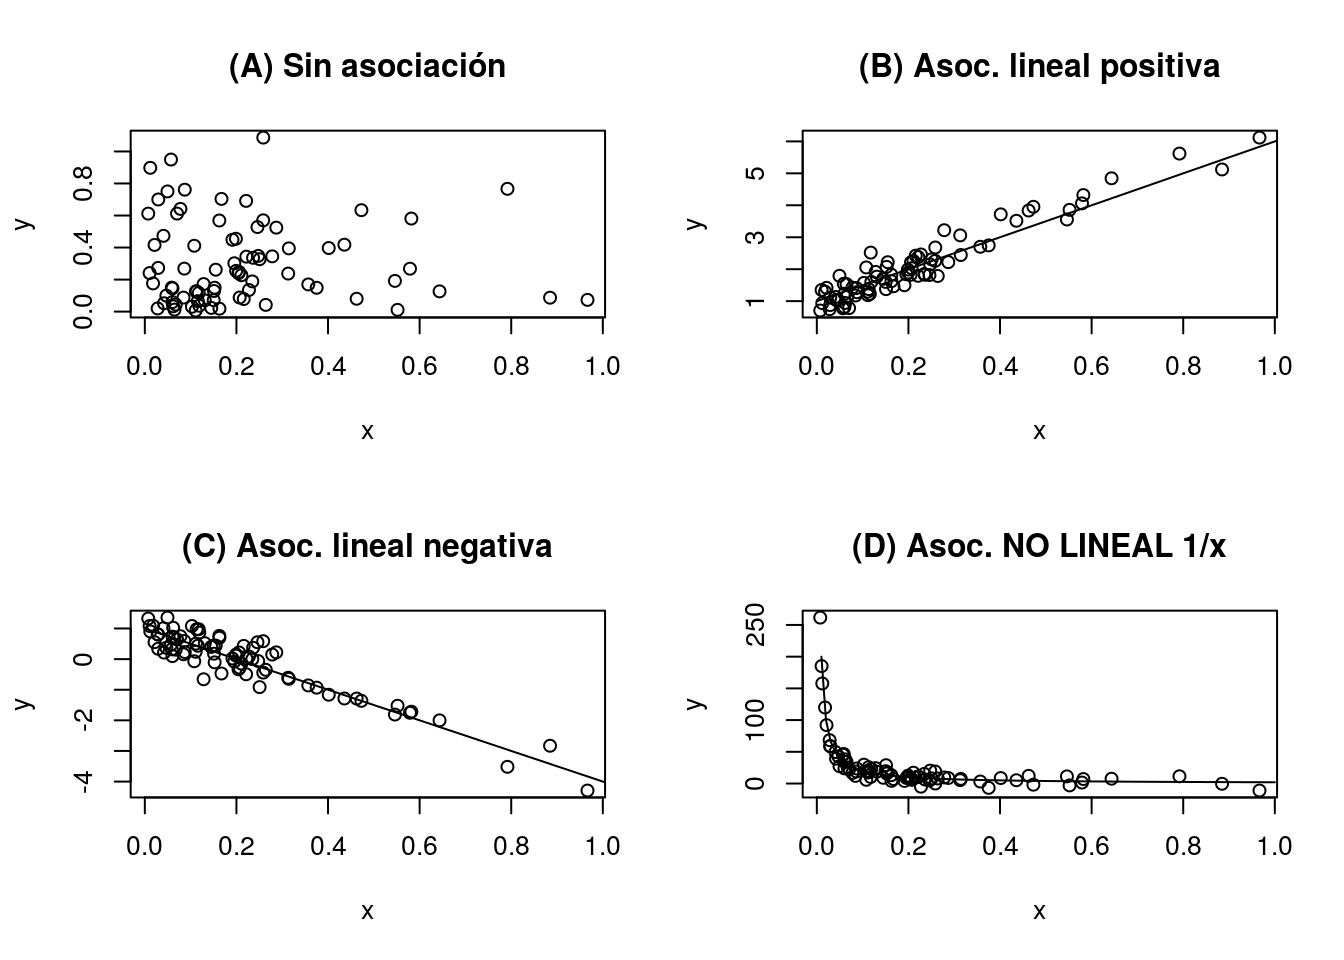
\includegraphics{Introduccion_prob_estad_bookdown_files/figure-latex/unnamed-chunk-103-1.pdf}

Notamos una asociación lineal entre mpg (millas
recorridas por galón lleno) y drat\footnote{La relación del eje
  es el número de revoluciones que el eje de salida o el
  eje de transmisión necesita hacer para hacer girar el
  eje una vuelta completa.} (revoluciones del eje)la
cual exploramos
de forma especifica a seguir.

\begin{verbatim}
## `geom_smooth()` using formula 'y ~ x'
\end{verbatim}

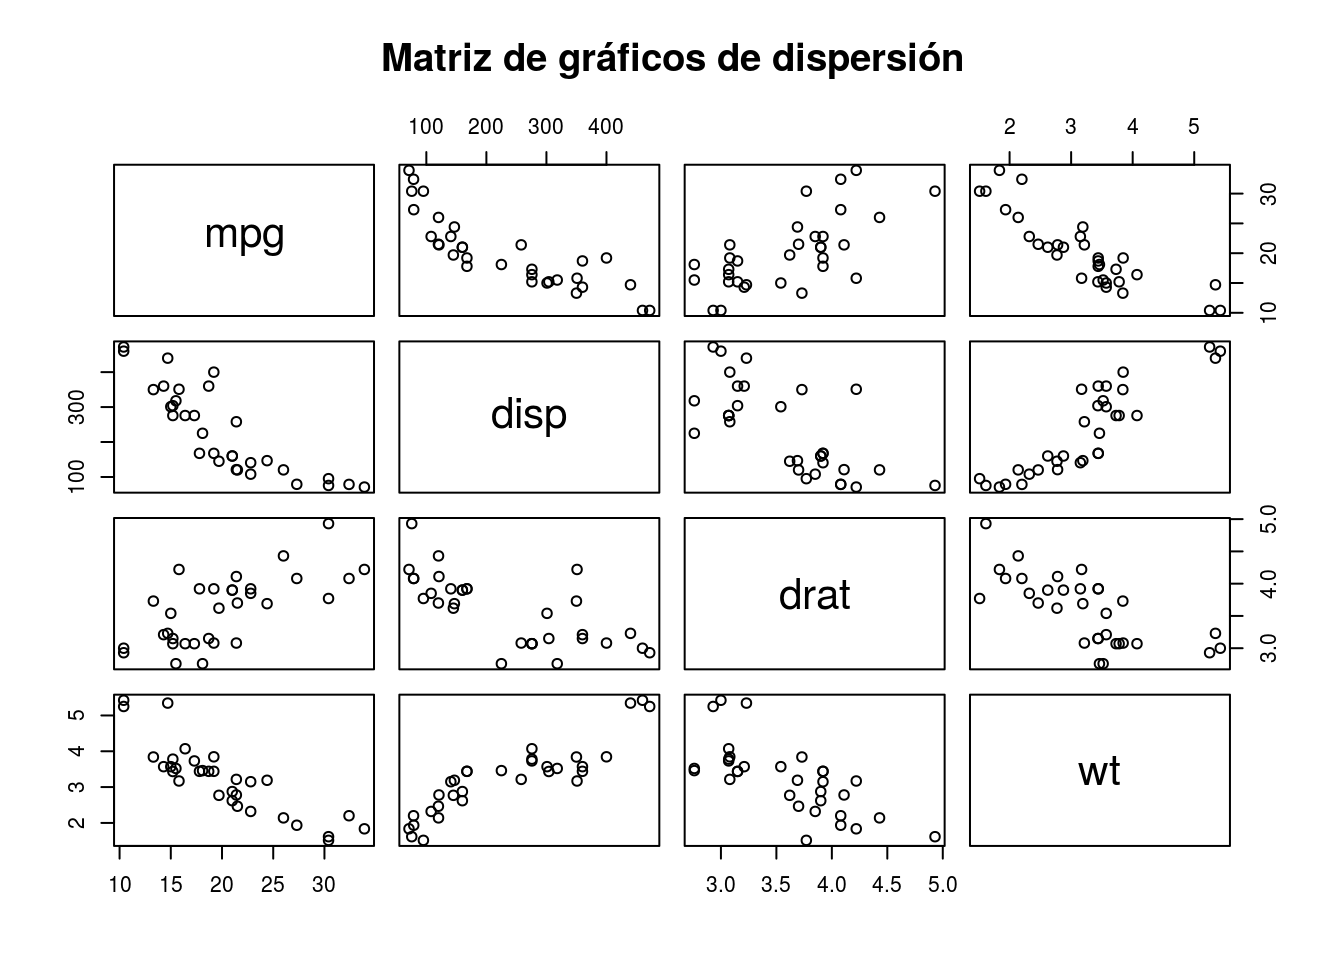
\includegraphics{Introduccion_prob_estad_bookdown_files/figure-latex/unnamed-chunk-104-1.pdf}

Unos de los objetivos consiste en determinar la
fórmula de la
recta que pasa por ``en medio de los puntos''.

\hypertarget{medidas-de-asociaciuxf3n-entre-dos-variables}{%
\section{Medidas de asociación entre dos variables}\label{medidas-de-asociaciuxf3n-entre-dos-variables}}

\begin{definition}
\protect\hypertarget{def:unnamed-chunk-105}{}{\label{def:unnamed-chunk-105} }Sea \(\bar{x}_n\) y \(\bar{y}_n\) la
media de los datos observados de X e Y,
respectivamente. La
covarianza entre estas dos variables es un
número que se denota por cov\((x,y)\) calculado por:

\[ \operatorname{cov}(x,y)=\frac{1}{n}\sum_{i=1}^
{n}\left(x_{i}-
 \bar{x}\right)\left(y_{i}-\bar{y}\right). \]
\end{definition}

\begin{definition}
\protect\hypertarget{def:unnamed-chunk-106}{}{\label{def:unnamed-chunk-106} }El \textbf{coeficiente de correlación muestral} entre
estas dos
variables \(X\) e \(Y\) es un número que se denota
por \(r(x, y)=r\).
Este
coeficiente se define de la siguiente forma.
\[r(x,y)= r =\frac{\operatorname{cov}(x,y)}{\sqrt
  { s_x^2  \times s_y^2}} \mbox{ donde
    } -1 < r < 1.\]
El coeficiente \(r\) mide la asociación lineal entre
los datos
observados de \(X\) e \(Y\).
Si \(r = 0\), decimos que \textbf{no existe} asociación
lineal entre
los datos. Si \(r<0\), decimos que existe una
\textbf{correlaciónlineal
negativa} o inversamente proporcional entre los
datos. Si, \(r > 0\), decimos que existe una \textbf{correlación lineal
positiva} entre
los datos o directamente proporcional.
\end{definition}

\begin{example}
\protect\hypertarget{exm:unnamed-chunk-107}{}{\label{exm:unnamed-chunk-107} }
Para los datos de mpg y drat, la covariancia es
\(2.20\) y el
coeficiente \(r=0.68\) es decir existe una
asociación lineal
positiva (o directamente proporcional) en mpg y
drat.
Interpretación: si los valores de mpg crecen,
también lo hace
drat. Si los valores de mpg decrecen, también lo
hacen drat.
\end{example}

\hypertarget{recta-media-estimada}{%
\section{Recta media estimada}\label{recta-media-estimada}}

Consideremos un par de variables, una de las
cuales será denominada variable de entrada, y la
otra, variable de respuesta.
Supongamos que para un valor dado, \(x\), de la
variable de
entrada, la variable de respuesta, \(y\), se puede
expresar en la forma

\[ Y = \beta_0 + \beta_1 x + e.\]
Los coeficientes \(\beta_0\) y \(\beta_1\) son
llamados los
parámetros del modelo. Se asume que la variable
\(e\), denominada
error aleatorio, es una variable aleatoria con
media \(0\), es
decir, asume valores muy cercano a \(0\).

\begin{definition}
\protect\hypertarget{def:unnamed-chunk-108}{}{\label{def:unnamed-chunk-108} }La relación entre la variable de \textbf{\emph{respuesta
(dependiente,output)}}, \(Y\), y la variable de
\textbf{\emph{entrada
(independiente, input)}}, \(x\), especificadas
ambas en la anterior
ecuación, se denomina regresión lineal simple.
\end{definition}

Para los pares de datos dados \((x_i, y_i), i = 1, . . . , n,\) los
estimadores de (por) mínimos cuadrados son los
valores de
\(\beta_0\) y \(\beta_1\) que hacen lo más pequeño
posible.

\[ \sum_{i=1}^{n}
\epsilon_{i}^{2}=\sum_{i=1}^{n}\left(y_{i}-
\beta_0-\beta_1
x_{i}\right)^{2} \]

lo más pequeño posible.

Se puede demostrar que los estimadores de mínimos
cuadrados de
\(\beta_0\) y \(\beta_1\) dados por

\[
\hat{\beta}_0=\frac{\sum_{i=1}^{n}\left(x_{i}-
\bar{x}\right)\left(y_
{i}-\bar{y}\right)}{\sum_{i=1}^{n}\left(x_{i}-
\bar{x}\right)^{2}}
\text{ y } 
\hat{\beta}_1=\bar{y}-\hat{\beta} \bar{x}
\]

\begin{definition}
\protect\hypertarget{def:unnamed-chunk-109}{}{\label{def:unnamed-chunk-109} }La recta
\[ \widehat{y} = \widehat{\beta}_0 +
\widehat{\beta}_1x.\]
se denomina \textbf{recta de regresión media estimada}:
\(\widehat{\beta}_1\) es la pendiente y
\(\widehat{\beta}_0\) es el
intercepto constante (o término independiente) de
la recta.
\end{definition}

\textbf{Interpretación:} Para valores cercanos a cero
de \(x\), observamos un valore medio cercano a
\(\widehat{\beta_0}\) de \(y\). Por cada incremento
(o decrecimo) de \(x\), observamos un incremento (o
decrecimo) medio de \(\widehat{\beta_1}\) unidades
en \(y\).

Preveer una nueva observación de las variables respuesta
\(y_{n+1}\) dado una variable de entrada \(x_{n+1}\) es
posible directamente simplemente evaluando la ecuación
de la recta, es decir:

\[ \widehat{y}_{n+1} = \widehat{\beta}_0 +
\widehat{\beta}_1x_{n+1}.
\]

\hypertarget{diagnostico-de-la-recta-lineal}{%
\section{Diagnostico de la recta lineal}\label{diagnostico-de-la-recta-lineal}}

\hypertarget{anuxe1lisis-de-asociaciuxf3n-entre-variables-categuxf3ricas}{%
\section{Análisis de asociación entre variables categóricas}\label{anuxe1lisis-de-asociaciuxf3n-entre-variables-categuxf3ricas}}

\begin{definition}
\protect\hypertarget{def:unnamed-chunk-110}{}{\label{def:unnamed-chunk-110} }Una \textbf{tabla de contingencia:} contiene las frecuencias
conjuntas observadas en la muestra de pares de atributos
expresadas por las unidades muestrales.
\end{definition}

Presentamos ejemplos de dos formas que podria tomar una
tabla de contingencia de dimensión \(2\times 3\).

\begin{table}[!htbp]
\centering
\caption{Tabla en frecuencia absoluta}
\label{mm}
\begin{tabular}{|l|l|l|l|l|}
\hline
s/r  &                 &  &  & \mbox{Suma}  \\ \hline
  &        $N_{11}$ & $N_{12}$  & $N_{13}$  & $N_{1+}$  \\ \hline
 &        $N_{21}$ & $N_{22}$  & $N_{23}$  &  $N_{2+}$ \\ \hline
\mbox{Suma} & $N_{+1}$ & $N_{+2}$ & $N_{+3}$  &  n \\ \hline
\end{tabular}
\end{table}

\begin{table}[!htbp]
\centering
\caption{Tabla en frecuencia relativa}
\label{m}
\begin{tabular}{|l|l|l|l|l|}
\hline
  s/r&                 &  &  & \mbox{Suma}  \\ \hline
   &        $p_{11}$ & $p_{12}$  & $p_{13}$  &  $p_{1+}$ \\ \hline
 &        $p_{21}$ & $p_{22}$  & $p_{23}$  & $p_{2+}$  \\ \hline
\mbox{Suma} & $p_{+1}$ & $p_{+2}$    & $p_{+3}$  & 1  \\ \hline
\end{tabular}
\end{table}

\textbf{Relación entre categorias de variables nominales}: la probabilidad de que una categria \(A\) ocurra es condicional (depende) o no depende (independiente) de otra categoria \(B\).

\begin{definition}
\protect\hypertarget{def:unnamed-chunk-111}{}{\label{def:unnamed-chunk-111} }Estadística \textbf{chi-cuadrado} es dada por para una tabla de congencia de
\(2\times 3\) es dada por:

\begin{equation*}
 Q= \sum_{i=1}^2 \sum_{j=1}^3 \frac{(N_{ij} - np_{i+}p_{+j})^2
  }{np_{i+}p_{+j} }
\end{equation*}

en que \(Q>0\).

\textbf{Coeficiente de contingencia} de Pearson es dado por:

\begin{equation*}
C= \sqrt{  \frac{Q}{Q+n}}  \in \left[0, \sqrt{\frac{k-1}{k}} \right]
\mbox{en que } k = \min \{s,r \} .
\end{equation*}
\end{definition}

\begin{definition}
\protect\hypertarget{def:unnamed-chunk-112}{}{\label{def:unnamed-chunk-112} }
\textbf{Coeficiente de contingencia} de Pearson CORREGIDO es dado por:

\begin{equation*}
C^{\prime}= \sqrt{\frac{k}{k-1}}\times C \in [0,1].
\end{equation*}

Un \(C^{*}\) cercano a \(0\) indica características independientes. \(C'\)
cerca de \(1\) señala una mayor medida de dependencia entre las
características.
\end{definition}

\begin{example}
\protect\hypertarget{exm:unnamed-chunk-113}{}{\label{exm:unnamed-chunk-113} }
Consideremos la base de datos \emph{mtcars} y las variables nominales
vs (tipo de motor en forma de v o recto) y am (cambio automatico o
manual).
Para este caso obtenemos un \(C^{*}=0.235\). Es decir, la probabilidad
de que un auto escogido al
azar sea automatico o
mecánico no depende de
la forma desu motor.
\end{example}

\hypertarget{ejercicios}{%
\section{Ejercicios}\label{ejercicios}}

\begin{enumerate}
\def\labelenumi{\arabic{enumi}.}
\item
  texto.
\item
  texto.
\item
  Texto.
\end{enumerate}

\hypertarget{prob}{%
\chapter{Evento aleatório}\label{prob}}

\hypertarget{operaciones-con-eventos-posibles-de-experimentos}{%
\section{Operaciones con eventos posibles de experimentos}\label{operaciones-con-eventos-posibles-de-experimentos}}

\begin{definition}
\protect\hypertarget{def:unnamed-chunk-114}{}{\label{def:unnamed-chunk-114} }
\textbf{Experimento científico}: es un experimento que se
ejecuta controlando
las circunstancias del entorno de manera de que este sea
\textbf{replicable} y
que las propiedades de los resultados posibles se
mantengan constantes.
\end{definition}

\begin{definition}
\protect\hypertarget{def:unnamed-chunk-115}{}{\label{def:unnamed-chunk-115} }
El \textbf{espacio muestral} de un experimento es el conjunto
(propuesto por el
investigador) que incluye todos los posibles resultados
de un experimento. Un caso que forma parte del espacio
muestral es llamado de \textbf{evento posible} del
experimento.
Un \textbf{evento elemental} es un evento mínimo que puede de
ocurrir.
\end{definition}

\begin{example}
\protect\hypertarget{exm:unnamed-chunk-116}{}{\label{exm:unnamed-chunk-116} }
Considere el experimento que consiste en lanzar un dado de seis caras al
aire sobre una superficie plana y observar la cara superior para registrar
el número que muestre. Incertidumbre: el dado podría mostrar un número del
uno al seis. El espacio muestral son los números del \(1\) al \(6\). Ejemplo
de eventos obtenemos un número par, obtenemos un número impar, obtenemos
un 5 y obtenemos un múltiplo de \(3\). Un evento imposible seria
obtenemos un número mayor a 7. Un evento elemental es obtenemos el número \(5\).
\end{example}

Una herramienta para representar eventos de un experimento es la teoría
ingenua de conjuntos. Usaremos la letra \(S\) para representar el espacio
muestral. Un evento elemental es simbolizado por \(\omega \in S\). Un evento
\(A\) del experimento será un subconjunto de \(S\), es decir \(A\subseteq S\).
Los eventos se pueden describir por \emph{extensión} o por \emph{comprensión}.

Presentamos un ejemplo:

\begin{example}
\protect\hypertarget{exm:unnamed-chunk-117}{}{\label{exm:unnamed-chunk-117} }
- Por compresión: \(\omega\in S\) tal que \(\omega=1,\ldots, 6\). Un evento
\(\omega \in A\) siempre que \(\omega=2,4,6\) (números pares). Evento elemental
\(\omega \in B\) siempre que \(\omega=5\). Otra forma de escribir \(S\) por comprensión es

\[S =\{\omega: \omega=1,\ldots,6 \} . \]

\begin{itemize}
\tightlist
\item
  Por extensión: \(S=\{1,2,3,4,5,6\}\), \(A= \{2, 4, 6 \}\) y \(B=\{5\}\).
\end{itemize}
\end{example}

Operaciones con eventos (conjuntos). Las operaciones de eventos de un
experimento son transformaciones de uno o más eventos en otros eventos del
experimento. Consideramos las siguientes:

\begin{itemize}
\tightlist
\item
  La union de \(A\) y \(B\), simbolizado por \(A\cup B\), transforma \(A\) y \(B\) en
  el evento \(A\cup B\) que contiene todos los eventos elementales de \(A\) y
  \(B\) juntos. Es decir,
\end{itemize}

\[A \cup B = \{\omega \in S: \omega \in A \mbox{ o también } \omega \in B
\}. \]

\begin{itemize}
\tightlist
\item
  La intersección de \(A\) y \(B\), simbolizado por \(A \cap B\), transforma \(A\)
  y \(B\) en el evento \(A\cap B\) que contiene todos los eventos elementales
  en común de \(A\) y \(B\).
\end{itemize}

\[A \cap B = \{\omega \in S: \omega \in A \mbox{ y a su vez } \omega \in B
\}. \]

\begin{itemize}
\tightlist
\item
  El complemento de A, simbolizado por \(A^c\), transforma \(A\) en el evento
  \(A^c\) que contiene todos los eventos elementales que no están en \(A\), pero
  si están en \(S\).
\end{itemize}

\[ A^c = \{\omega\in S: \omega \notin A \}. \]

\begin{definition}
\protect\hypertarget{def:unnamed-chunk-118}{}{\label{def:unnamed-chunk-118} }
Una lista \(A_1, \ldots, A_k\) de eventos de \(S\) , simbolizada por
\(\mathcal{A}\) es llamada de una \textbf{clase de eventos} de \(S\).
La clase \(\mathcal{A}\) es una álgebra de sucesos si cumple las siguientes
condiciones:

\begin{itemize}
\item
  \(S \in \mathcal{A}\).
\item
  Todas las uniones finitas de eventos de \(S\) estan también en \(S\).
\item
  El complemento de todos los eventos de \(S\) también están en \(S\).
\end{itemize}
\end{definition}

\begin{definition}
\protect\hypertarget{def:unnamed-chunk-119}{}{\label{def:unnamed-chunk-119} }Sigma álgebra de Borel (pendiente).
\end{definition}

\hypertarget{medida-de-probabilidad-y-experimentos-aleatorios}{%
\section{Medida de probabilidad y experimentos aleatorios}\label{medida-de-probabilidad-y-experimentos-aleatorios}}

\begin{definition}
\protect\hypertarget{def:unnamed-chunk-120}{}{\label{def:unnamed-chunk-120} }
Sea \(\mathcal{A}\) una álgebra de eventos de \(S\). Una función \(\mbox{Pr}: \mathcal{A}\to [0,1]\) que le asigna a cada evento de \(\mathcal{A}\) un
número dentro del intervalo \([0,1]\) es llamada de \textbf{medida de
probabilidad finita} siempre que satisfaga las siguientes condiciones:

\begin{itemize}
\item
  1 \(\mbox{Pr}(A)\geq 0\).
\item
  2 \(\mbox{Pr}(S) =1\).
\item
  3 \(A_1,\ldots, A_n\in \mathcal{A}\) disjuntos (\(2\) a \(2\)), entonces

  \[ \mbox{Pr}\left(\bigcup_{k=1}^{n} A_k \right)=
  \sum_{k=1}^{n}\mbox{Pr}(A_k). \]
\end{itemize}
\end{definition}

Una medida de probabilidad es una operación que mide la incertidumbre del
evento \(A\) en un número en \([0,1]\). Esta medida le da el máximo valor
al espacio muestral. La suma de probabilidades de eventos disjuntos es la
probabilidad de las uniones.

Propiedades de la medida de probabilidad. Una medida de probabilidad que
satisface 1 a 3 satisface las siguientes propiedades:

\begin{itemize}
\tightlist
\item
  Pr\((A \cup B)\)= Pr\((A)\)+ \(\mbox{Pr}(B)\) - Pr\((A\cap B)\).
\item
  Pr\((A^c)= 1-\mbox{Pr}(A)\).
\end{itemize}

\begin{definition}
\protect\hypertarget{def:unnamed-chunk-121}{}{\label{def:unnamed-chunk-121} }
Sea \(A\) un evento de un experimento con espacio muestral \(S\) de
con un número de eventos elementales finito. Se define la \textbf{probabilidad
clásica} del evento \(A\) como
el cociente

\[\mbox{Pr}(A)=\frac{ \mbox{Número de casos a favor de } A}{ \mbox{Número
  de casos totales (a favor de $S$)}}.\]

Este cálculo de probabilidad también es conocida como la \textbf{regla de
Laplace}.
\end{definition}

\textbf{Principio de razón insuficiente:} sino tenemos información previa o no
queremos asumir un sesgo personal sobre la incertidumbre de una propiedad
muestral, entonces debemos asignar la \emph{misma probabilidad} a cada evento
puntual de \(\Omega\). La medida de probabilidad de un evento \(A\) es la razón
entre el número de casos a favor de \(A\) y el número tal de casos posibles.

\begin{definition}
\protect\hypertarget{def:unnamed-chunk-122}{}{\label{def:unnamed-chunk-122} }
Un \textbf{modelo de probabilidad} para un experimento es
formado por el espacio muestral \(S\), una álgebra
\(\mathcal{A}\) de eventos de \(S\) y
una medida de probabilidad de Pr. Esto puede ser
representado por la tripla \((S, \mathcal{A}, \mbox{Pr})\)

Un \textbf{experimento aleatorio} es un \emph{experimento} si y
solmente si en cuya construcción tiene asociado una
medida de probabilidad
para sus eventos.
\end{definition}

\hypertarget{interpretaciuxf3n-frecuentista-de-una-medida-de-probabilidad}{%
\subsection{Interpretación frecuentista de una medida de probabilidad}\label{interpretaciuxf3n-frecuentista-de-una-medida-de-probabilidad}}

Supongamos que repetimos un mismo experimento
secuencialmente. Los primeros \(n\) resultados posibles
son representados por \(\omega_1 , \omega_2, \ldots, \omega_n\) y que \(\mathbb{I}_A (\omega_i)= 1\)
cuando \(\omega_i \in A\). Luego, según la interpretación
frecuentista, para un máximo de diferencia absoluta
\(\epsilon\) siempre va a existir un momento de repetición
\(n_0\) del experimento tal que:

\[\big | 1/n\sum_{i=1}^{n} \mathbb{I}_A(\omega_i) -
\mbox{Pr}(A)\big |
< \epsilon, \forall n\geq n_0\].

Es decir, a partir de una repetición finita del
experimento, la diferencia entre \(\mbox{Pr}(A)\) y
\(1/n\sum_{i=1}^{n} \mathbb{I}_A(\omega_i)\) es tan
pequeña
como querramos. Es decir Pr\((A)\) es el \textbf{límite de las
frecuencias relativas} de observar eventos elementales
de \(A\) en la replicación secuencial de un mismo
experimento.

\hypertarget{propiedades-buxe1sicas-de-la-medida-de-probabilidad}{%
\section{Propiedades básicas de la medida de probabilidad}\label{propiedades-buxe1sicas-de-la-medida-de-probabilidad}}

\begin{definition}
\protect\hypertarget{def:unnamed-chunk-123}{}{\label{def:unnamed-chunk-123} }Probabilidad conjunta, marginal y condicional.
\end{definition}

\begin{definition}
\protect\hypertarget{def:unnamed-chunk-124}{}{\label{def:unnamed-chunk-124} }Eventos estocasticamente independientes.
\end{definition}

\begin{definition}
\protect\hypertarget{def:unnamed-chunk-125}{}{\label{def:unnamed-chunk-125} }Probabilidad total.
\end{definition}

\begin{definition}
\protect\hypertarget{def:unnamed-chunk-126}{}{\label{def:unnamed-chunk-126} }Teorema de Bayes.
\end{definition}

\hypertarget{resultados-buxe1sicos-de-combinatoria}{%
\section{Resultados básicos de combinatoria}\label{resultados-buxe1sicos-de-combinatoria}}

\begin{definition}
\protect\hypertarget{def:unnamed-chunk-127}{}{\label{def:unnamed-chunk-127} }Principio básico del conteo.
\end{definition}

\begin{definition}
\protect\hypertarget{def:unnamed-chunk-128}{}{\label{def:unnamed-chunk-128} }Principio básico del conteo generalizado.
\end{definition}

\hypertarget{var}{%
\chapter{VARIABLES ALEATORIAS Y SUS DISTRIBUCIONES}\label{var}}

\hypertarget{elementos-buxe1sicos}{%
\section{Elementos básicos}\label{elementos-buxe1sicos}}

\begin{definition}
\protect\hypertarget{def:unnamed-chunk-129}{}{\label{def:unnamed-chunk-129} }Sea \(S\) el espacio muestral de un experimento. Una función \(X\) con valores reales que le otorga a cada elemento de \(S\) un valor numérico es \textbf{variable aleatoria}. El conjunto de todos los valores posibles que puede asumir \(X\) es llamado de espacio muestral de \(X\) y es denotado por \(\mathcal{X}\). Usaremos la notación \(X:S\to \mathcal{X}\).
\end{definition}

\begin{example}
\protect\hypertarget{exm:unnamed-chunk-130}{}{\label{exm:unnamed-chunk-130} }
- \(X_1\): número de caras que resultan al lanzar \(10\) veces un
monedas al aire.

\begin{itemize}
\item
  \(X_2\): el número de seis al lanzar un dado \(15\) veces.
\item
  \(X_3\): el número de accidentes por semana que ocurren una
  empresa.
\item
  \(X_4\): el consumo de leña por casas en una ciudad.
\end{itemize}
\end{example}

\begin{definition}
\protect\hypertarget{def:unnamed-chunk-131}{}{\label{def:unnamed-chunk-131} }
La función de densidad \(f\) para una variable aleatoria
continua \(X\) cuyo espacio muestral es \(\mathcal{X}\) es
una función que modela la variabilidad de los posibles
valores de \(X\) y nos ayuda a calcular la probabilidad de
que ella asuma determinados valores. Esta función
satisface las siguientes propiedades.

\begin{itemize}
\tightlist
\item
  \(f(x)\geq 0\) para todo \(x\).
\item
  \(\int_{\mathcal{X}}f(x)dx=1\).
\end{itemize}

La probabilidad de que \(X\in (a,b)\) es el área bajo la
curva de \(f\) limitado al intervalo \((a,b)\).
\end{definition}

\begin{definition}
\protect\hypertarget{def:unnamed-chunk-132}{}{\label{def:unnamed-chunk-132} }
Por otro lado, la función de probabilidad \(p\) para una
variable aleatoria discreta \(X\) cuyo espacio muestral es
\(\mathcal{X}\) es una función que modela la variabilidad
de los posibles valores de \(X\) y nos ayuda a calcular la
probabilidad de que ella asuma determinados valores.
Esta función satisface las siguientes propiedades.

\begin{itemize}
\tightlist
\item
  \(p(x)\geq 0\) para todo \(x\).
\item
  \(\sum_{x\in \mathcal{X}}p(x)=1\).
\end{itemize}

La probabilidad de que \(X\in \{a_1, \ldots, a_k \}\) es
la suma \(\sum_{x \in \{a_1, \ldots, a_k \}}p(x)\).
\end{definition}

\begin{example}
\protect\hypertarget{exm:unnamed-chunk-133}{}{\label{exm:unnamed-chunk-133} }
Consideremos la función de densidad \(f\) dada por
\[f(x)= \frac{1}{\pi(1+x^2)}, \quad x\in R, \]

en que \(\pi\) es la constante pi.

La función de densidad \(p\) dada por
\[p(x)=(1-1/6)^{x-1}1/6, \quad x=1,2,\ldots. \]
\end{example}

Cuando \(f\) o \(p\) esta totalmente especificada, ambas son
llamados de \textbf{modelo de probabilidad} para \(X\). Cuando \(f\) o
\(p\) depende una constante \(\theta\) asumida como
desconocida, entonces ellas son llamadas de \textbf{modelo
estadístico} para \(X\). El objetivo de los métodos de
inferencia es determinar valores plausibles de \(\theta\)
desde una muestra observada.

En el último caso \(f(x)\) es representada por
\(f(x;\theta)\) indicando que \(f\) es una función de \(x\)
para un valor de \(\theta\) que debe ser especificado. En el
caso discreto, \(p(x)\) es representado por \(p(x;\theta)\).

\begin{definition}
\protect\hypertarget{def:unnamed-chunk-134}{}{\label{def:unnamed-chunk-134} }
La función de distribución acumulada de una variable
aleatoria \(X\) es la funcion \(F(x)= \mbox{Prob}(X\leq x)\), en
el caso
continuo, es definida por
\[ F(x)= \int_{-\infty}^x f(t;\theta)dt \]
y en el caso discreto
\[ F(x)=\sum_{t=-\infty}^{x}p(t;\theta).\]

Propiedades de \(F(x)\):

\begin{itemize}
\tightlist
\item
  Pr\((a<X<b) = F(b)- F(a)\),
\item
  Pr\((X>a) = 1- F(a)\),
\item
  \(\lim_{x\to + \infty}F(x) =1\),\\
\item
  \(\lim_{x\to - \infty}F(x)=0\).
\end{itemize}
\end{definition}

\begin{example}
\protect\hypertarget{exm:unnamed-chunk-135}{}{\label{exm:unnamed-chunk-135} }Para la función f y P antes presentadas, las respectivas funciones de
probabilidad acumulada son,

\[F(x)= \int_{-\infty}^{x} \frac{1}{\pi(1+t^2)} dt \]
y
\[ F(x)= \sum_{t= 0}^{x} (1-\pi)^{t-1}\pi  \]

respectivamente.
\end{example}

\begin{definition}
\protect\hypertarget{def:unnamed-chunk-136}{}{\label{def:unnamed-chunk-136} }
Una variable aleatoria \(X\) es \textbf{discreta} si el conjunto de
sus posibles
resultados \(\mathcal{X}\) es finito o puede ser enumerados en
la forma
\(\{a_1,a_2,\ldots, a_n, \ldots\}\). Una variable aleatoria \(X\)
es \textbf{continua} si existe una función de densidad para ella.
\end{definition}

\hypertarget{distribuciones-de-probabilidad-de-variables-aleatorias-discreta}{%
\section{Distribuciones de probabilidad de variables aleatorias discreta}\label{distribuciones-de-probabilidad-de-variables-aleatorias-discreta}}

\begin{definition}
\protect\hypertarget{def:unnamed-chunk-137}{}{\label{def:unnamed-chunk-137} }
Una variable aleatoria \textbf{Bernoulli} es una indicadora de la
ocurrencia de evento \(A \subseteq S\). Es decir, \(X=1\) cuando
\(\omega \in A\) (ocurre \(A\)) con probabilidad \(p\) y \(X=0\)
cuando \(\omega \notin A\) (no ocurre \(A\)) con probabilidad
\(p\). Esto se representa por \(X \sim \mbox{Bernoulli}(p)\).

La función de probabilidad de \(X\) es:
\[p(x;\theta)= \theta^{x}(1-\theta)^{x-1} \mbox{ para } x=0,1
  \mbox{ y } \theta \in (0,1). \]
\end{definition}

\begin{example}
\protect\hypertarget{exm:unnamed-chunk-138}{}{\label{exm:unnamed-chunk-138} }
Consideremos el experimento del lanzamiento de una moneda al
aire. Sea \(X=1\) cuando obtenemos una cara con
probabilidad \(p=1/2\) y \(X=0\) cuando obtenemos un sello con
probabilidad \(1-1/2\).

Consideremos el experimento del lanzamiento de un dado al
aire. Sea \(X=1\) cuando obtenemos una seis con
probabilidad \(p=1/6\) y \(X=0\) cuando no con
probabilidad \(1-1/6\).
\end{example}

\begin{definition}
\protect\hypertarget{def:unnamed-chunk-139}{}{\label{def:unnamed-chunk-139} }
Considere una repetición de mismo experimento \(n\) y sea
\(X_1, X_2, \ldots,X_n\) una secuencia independiente de
variables Bernoulli, en que \(X_i=1\) cuando \(\omega \in A\) con
probabilidad \(\theta\) para \(i=1, \ldots, n\). Una variable
\textbf{Binomial} \(Z\) es el número de caso a favor de \(A\) al
repetir el experimento \(n\) veces, es decir:

\[ Z = \sum_{i=1}^n X_i . \]

Esto se representa por \(Z \sim \mbox{Binomial}(n,\theta)\). Su
función de probabilidades es:

\[ p(z;n,\theta)=\frac{n!}{z!(n-z)!}\theta^{z}(1-\theta)^{n-
    z}.    \]
\end{definition}

\begin{example}
\protect\hypertarget{exm:unnamed-chunk-140}{}{\label{exm:unnamed-chunk-140} }
En primer caso, considere el experimento de lanzar una moneda
\(n=15\) veces y observar los lanzamientos de cara. Sea
\(X_1=x_1,\ldots, X_n=x_n\) las indicadoras de observar este
evento en cada repetición. Luego \(Z= \sum_{i=1}^{15}x_i\) es
el número de caras observar al lanzar la moneda \(15\) veces.
En este caso \(Z \sim \mbox{Binomial}(15, 1/2)\)

En segundo caso, considere el experimento de lanzar un dado
\(n=20\) veces y observar los números un seis. Sea
\(X_1=x_1,\ldots, X_n=x_n\) las indicadoras de observar este
evento en cada repetición. Luego \(Z= \sum_{i=1}^{20}x_i\) es
el número de seis que observamos al lanzar el dado \(20\)
veces. En este caso \(Z \sim \mbox{Binomial}(20, 1/6)\).
\end{example}

\begin{example}
\protect\hypertarget{exm:unnamed-chunk-141}{}{\label{exm:unnamed-chunk-141} }
Distribución multinomial (pendiente).
\end{example}

\begin{example}
\protect\hypertarget{exm:unnamed-chunk-142}{}{\label{exm:unnamed-chunk-142} }
Cuando \(X\) es una variable que mide el número eventos que
ocurren en un determinado intervalo de tiempo \([c,c+t]\) de
longitud \(t\). Sobre ciertas suposiciones, una de las opciones es
el modelo de \textbf{Poisson} con un promedio de ocurrencias por
intervalo igual a \(\lambda\).

Una variable Poisson tiene función de probabilidad dada por:

\[ p(x;\lambda)=\frac{ \mbox{e}^{-\lambda}\lambda^{x} }{x!}
   \mbox{ para } x\in \mathbb{N} \mbox{ y } \lambda >0. \]

y función de distribución acumulada dada por:

\[F(x; \lambda)= \sum_{k=0}^{x}
  \frac{\mbox{e}^{-\lambda}\lambda^{k}}{k!}.   \]
\end{example}

\begin{example}
\protect\hypertarget{exm:unnamed-chunk-143}{}{\label{exm:unnamed-chunk-143} }
- \(X\): número de accidentes por semana que ocurren en una
industria papelera. Para \(\lambda=3\), si observamos repetidas
observaciones de \(X\), luego observaríamos en promedio \(3\)
accidentes por semana.

\begin{itemize}
\item
  \(X\): número de accidentes en una carretera por día. Para
  \(\lambda=4\), si observamos repetidas observaciones de \(X\), luego
  observaríamos \(4\) accidentes en la carretera por día.
\item
  \(X\): número de partículas por minuto que emite una
  sustancia radiactiva. Para \(\lambda=17\), si observamos
  repetidas observaciones de \(X\), luego observaríamos en promedio
  \(17\) partículas por minuto.
\end{itemize}
\end{example}

\begin{example}
\protect\hypertarget{exm:unnamed-chunk-144}{}{\label{exm:unnamed-chunk-144} }
Distribución geométrica (pendiente).
\end{example}

\begin{example}
\protect\hypertarget{exm:unnamed-chunk-145}{}{\label{exm:unnamed-chunk-145} }
Distribución binomial negativa (pendiente).
\end{example}

\begin{example}
\protect\hypertarget{exm:unnamed-chunk-146}{}{\label{exm:unnamed-chunk-146} }
Distribución hipergeométrica (pendiente).
\end{example}

\hypertarget{distribuciones-de-probabilidad-de-variables-aleatorias-continuas.}{%
\section{Distribuciones de probabilidad de variables aleatorias continuas.}\label{distribuciones-de-probabilidad-de-variables-aleatorias-continuas.}}

En esta sección presentamos algunos modelos para variables
aleatorias continuas.

\begin{example}
\protect\hypertarget{exm:unnamed-chunk-147}{}{\label{exm:unnamed-chunk-147} }
Una variable \(X>0\) sigue un modelo \textbf{Exponencial} con taza de
concentración \(1/\lambda\) cuando su función de densidad es dada
por:

\[ f(x;\lambda)= \lambda \mbox{e}^{-x\lambda}, \mbox{ para }
     x>0,\ \lambda>0.     \]

La taza de concentración \(1/\lambda\) indica el promedio de tiempo
medio de \(X\). El parámetro de decaimiento \(\lambda\) nos indica la
forma de la densidad en el sentido de que indica que tan rápido decae
(va hacia cero) la cola izquierda de \(f(x;\lambda)\).

Su función de probabilidad acumulada es dada por:

\[F(x;\lambda)= \int_{-\infty}^{x} \lambda \mbox{e}^{-t\lambda}dt=
    1- \mbox{e}^{-x\lambda}.   \]
\end{example}

\begin{example}
\protect\hypertarget{exm:unnamed-chunk-148}{}{\label{exm:unnamed-chunk-148} }
Una variable aleatoria se suele considerar Exponencial cuando esta
es contínua y mide el tiempo de ``vida'' o de ``duración'' de vida
útil de objetos. Por ejemplo:

\begin{itemize}
\item
  \(X\): tiempo de funcionamiento de una máquina procesadora
  de leche en miles de horas. Para \(\lambda= 1/10\), si
  observásemos repetidos tiempos de funcionamiento de
  muchas máquinas del mismo tipo, observaríamos un promedio
  de \(10\) mil horas.
\item
  \(X\): tiempo de vida de circuitos eléctricos en miles de horas.
  Para \(\lambda=1/5\), si observásemos repetidos
  tiempos de vida de circuitos, observaríamos un promedio
  de \(5\) mil horas.
\item
  \(X\): tiempos de llegada en minutos de clientes a una fila de
  banco. Para \(\lambda= 1/4\), si observásemos una gran
  cantidad de observaciones de esta, observaríamos un
  promedio de \(4\) minutos.
\end{itemize}
\end{example}

\begin{definition}
\protect\hypertarget{def:unnamed-chunk-149}{}{\label{def:unnamed-chunk-149} }
Una variable normal \(X\) se usa para modelar variables límites o
aproximadamente simetricas. Su función de densidad es dada por

\[ f(x;\mu, \sigma) =
\frac{1}{\sigma\sqrt{2\pi}}\exp\left[-\frac{(x -
\mu)^2}{2\sigma^2}  \right],  \]

donde \(\mu \in \mathbb{R}\) es el parámetro posición,
\(\sigma>0\) es la varianza y \(x\in \mathbb{R}\).
\end{definition}

\begin{example}
\protect\hypertarget{exm:unnamed-chunk-150}{}{\label{exm:unnamed-chunk-150} }
- \(X\): puntajes de pruebas estandarizadas.

\begin{itemize}
\tightlist
\item
  \(X\): promedios de variables con más de \(30\) datos observados.
\end{itemize}
\end{example}

\begin{example}
\protect\hypertarget{exm:unnamed-chunk-151}{}{\label{exm:unnamed-chunk-151} }Distribución Beta.
\end{example}

\begin{example}
\protect\hypertarget{exm:unnamed-chunk-152}{}{\label{exm:unnamed-chunk-152} }
Distribución Gumbel.
\end{example}

\begin{example}
\protect\hypertarget{exm:unnamed-chunk-153}{}{\label{exm:unnamed-chunk-153} }Distribución Weibull.
\end{example}

\begin{example}
\protect\hypertarget{exm:unnamed-chunk-154}{}{\label{exm:unnamed-chunk-154} }Distribución uniforme.
\end{example}

\hypertarget{varbi}{%
\chapter{DISTRIBUCIONES BIDEMENSIONALES}\label{varbi}}

\hypertarget{uno}{%
\section{Uno}\label{uno}}

\hypertarget{dos}{%
\section{Dos}\label{dos}}

\hypertarget{expected}{%
\chapter{VALOR ESPERADO}\label{expected}}

\begin{definition}
\protect\hypertarget{def:unnamed-chunk-155}{}{\label{def:unnamed-chunk-155} }Media y variancia poblacional.
\end{definition}

\begin{example}
\protect\hypertarget{exm:unnamed-chunk-156}{}{\label{exm:unnamed-chunk-156} }Ejemplos media y variancia poblacional.
\end{example}

\begin{definition}
\protect\hypertarget{def:unnamed-chunk-157}{}{\label{def:unnamed-chunk-157} }Función generadora de probabilidad y momentos.
\end{definition}

\hypertarget{valor-esperado-de-modelos-discretos}{%
\section{Valor esperado de modelos discretos}\label{valor-esperado-de-modelos-discretos}}

\hypertarget{valor-esperado-de-modelos-discretos-1}{%
\section{Valor esperado de modelos discretos}\label{valor-esperado-de-modelos-discretos-1}}

\hypertarget{ass}{%
\chapter{Resultados asintóticos.}\label{ass}}

\hypertarget{xmuestras}{%
\chapter{Variables aleatorias funciones de una muestra aleatoria}\label{xmuestras}}

\hypertarget{ejemplos-de-funciones-de-una-muestra-aleatoria}{%
\section{Ejemplos de funciones de una muestra aleatoria}\label{ejemplos-de-funciones-de-una-muestra-aleatoria}}

\begin{definition}
\protect\hypertarget{def:unnamed-chunk-158}{}{\label{def:unnamed-chunk-158} }
Una muestra aleatoria de tamaño \(n\) de un modelo de probabilidad cualquiera,
simbolizada por \(X_1,\ldots, X_n\), es una secuencia de variables aleatorias
en que (i) \(X_i\) sigue el mismo modelo en cuestion para \(i=1,\ldots,n\) y
(ii) \(X_i\) y \(X_j\) son independientes para cada \(i \neq j\).
\end{definition}

\begin{example}
\protect\hypertarget{exm:unnamed-chunk-159}{}{\label{exm:unnamed-chunk-159} }
Supongamos que lanzo \(n\) veces una moneda al aire tal que la probabilidad
\(\pi\) muestra cara. Simbolicemos por \(X_i=1\) cuando la moneda muestre cara
en el \(i\)-ésimo lanzamiento, para \(i=1,\ldots,n\). El resultado será una
muestra aleatoria de un modelo Bernoulli.

Una muestra aleatoria de tamaño \(n\) un modelo de
\(\mbox{Bernoulli}(\pi)\),
simbolizada por \(X_1,\ldots, X_n\), es una secuencia de variables aleatorias
en que (i) \(X_i \sim \mbox{Bernoulli}(\pi)\) para \(i=1,\ldots,n\) y (ii)
\(X_i\) y \(X_j\) son independientes para cada \(i \neq j\).
\end{example}

\begin{example}
\protect\hypertarget{exm:unnamed-chunk-160}{}{\label{exm:unnamed-chunk-160} }
Una muestra aleatoria de tamaño \(n\) un modelo de
\(\mbox{Normal}(\mu,\sigma^2)\),
simbolizada por \(X_1,\ldots, X_n\), es una secuencia de variables aleatorias
en que (i) \(X_i \sim \mbox{Normal}(\mu,\sigma^2)\) para \(i=1,\ldots,n\) y (ii)
\(X_i\) y \(X_j\) son independientes para cada \(i \neq j\).
\end{example}

\begin{definition}
\protect\hypertarget{def:unnamed-chunk-161}{}{\label{def:unnamed-chunk-161} }
Una variable aleatoria \(Z\) es una función de una muestra aleatoria
\(X_1,\ldots,X_n\) si \(Z\) se puede escribir como una función de esta, es
decir
\[ Z(X_1,\ldots,X_n) = \phi(X_1,\ldots,X_n),   \]
en que \(\phi(\dot)\) es una función de \(n\) variables.

La distribución o el modelo de probabilidad de \(Z\) es llamada (o) de
\textbf{distribución muestral}.
\end{definition}

Presentamos dos ejemplos de funciones de variables aleatorias.

\begin{example}
\protect\hypertarget{exm:unnamed-chunk-162}{}{\label{exm:unnamed-chunk-162} }
Sea \(X_1,\ldots, X_n\) una muestra aleatoria de tamaño \(n\) un modelo de
\(\mbox{Bernoulli}(\pi)\), luego

\[  Z= Z(X_1,\ldots,X_n)= \sum_{i=1}^{n}X_i \sim \mbox{Binomial}(n\pi).  \]
\end{example}

\hypertarget{variables-aleatorias-funciones-de-una-muestra-aleatoria-normal}{%
\section{Variables aleatorias funciones de una muestra aleatoria normal}\label{variables-aleatorias-funciones-de-una-muestra-aleatoria-normal}}

\begin{example}
\protect\hypertarget{exm:unnamed-chunk-163}{}{\label{exm:unnamed-chunk-163} }
Sea \(X_1,\ldots, X_n\) una muestra aleatoria de tamaño \(n\) un modelo de
\(\mbox{Normal}(\mu,\sigma^2)\), luego

\[  \bar{X}_n= \bar{X}_n(X_1,\ldots,X_n)= \frac{1}{n}\sum_{i=1}^{n}X_i \sim
  \mbox{Normal}(\mu, \sigma^2/n).  \]
\end{example}

\begin{definition}
\protect\hypertarget{def:unnamed-chunk-164}{}{\label{def:unnamed-chunk-164} }

Una variable aleatoria \textbf{chi-cuadrado} \(X\) tiene función de
densidad dada por:

\[ f(x ; \nu)=
\frac{x^{\frac{\nu}{2}-1} e^{-\frac{x}{2}}}{2^{\frac{\nu}{2}}
  \Gamma\left(\frac{\nu}{2}\right)},   \]
en donde el parámetro \(\nu\) es llamado de \textbf{grados de libertad} de
\(X\) y \(\Gamma(k)= \int_{0}^{\infty} x^{k-1}e^{-x} dx\) es la función
gamma. Esto es simbolizado por \(X \sim \chi^2_{\nu}\).
\end{definition}

\begin{example}
\protect\hypertarget{exm:unnamed-chunk-165}{}{\label{exm:unnamed-chunk-165} }
Considere una muestra aleatoria \(X_1,\ldots, X_n\) con modelo
\(\mbox{Normal}(\mu,\sigma^2)\), luego

\[\frac{(n-1)S^2}{\sigma^2} \sim \chi^2_{n-1}.\]

Luego, podemos calcular la probabilidad de eventos asociados a la variable
\(\frac{(n-1)S^2}{\sigma^2}\) cuando \(\sigma\) es conocido. En inferencia
clásica, es útil encontrar el intervalo de confianza para \(\sigma^2\) cuando
conocemos los cuantiles de orden \(\chi_{n-1,\alpha/2}\) y
\(\chi_{n-1,1-\alpha/2}\) tal que
\[ \mbox{Pr}\left(  \chi_{n-1,\alpha/2}^2 \leq \frac{(n-1)S^2}{\sigma^2}
\leq  \chi_{n-1,1-\alpha/2}^2 \right) =  1- \alpha.   \]

Luego,

\begin{eqnarray*}
\mbox{Pr}\left(  \chi_{n-1,\alpha/2}^2 \leq \frac{(n-1)S^2}{\sigma^2} \leq 
          \chi_{n-1,1-\alpha/2}^2 \right) &=& 
\mbox{Pr}\left(\frac{1}{ \chi_{n-1,\alpha/2}^2 } \geq 
                \frac{  \sigma^2}{(n-1)S^2}  \geq 
           \frac{1}{ \chi_{n-1,1-\alpha/2}^2 } \right) \\
&=& \mbox{Pr}\left(\frac{(n-1)S^2}{\chi_{n-1,\alpha/2}^2} \geq \sigma^2 
                    \geq 
           \frac{(n-1)S^2}{  \chi_{n-1,1-\alpha/2}^2 } \right)\\
&=& \mbox{Pr}\left(\frac{(n-1)S^2}{ \chi_{n-1,1-\alpha/2}^2} \leq \sigma^2 
                    \leq 
           \frac{(n-1)S^2}{ \chi_{n-1,\alpha/2}^2} \right)\\
&=& 1 - \alpha. 
\end{eqnarray*}

Luego, para \(\alpha= 0.05\) y \(n=30\), tenemos que \(\chi_{n-1,\alpha/2}^2=  16.05\) y \(\chi_{n-1,\alpha/2}^2= 45.72\) y \(s^2=34\), tenemos que:

\begin{eqnarray*}  
\mbox{Pr}\left(\frac{29*34}{ 45.72} \leq \sigma^2 
                    \leq 
             \frac{(29*34}{16.05}\right) 
&=& \mbox{Pr}\left( 21.57 \leq \sigma^2 
                    \leq  61.43 \right) \\
&=& 0.95 (95\%).  
\end{eqnarray*}
\end{example}

\begin{definition}
\protect\hypertarget{def:unnamed-chunk-166}{}{\label{def:unnamed-chunk-166} }Una variable aleatoria \(T\) tiene un modelo \textbf{t-student} cuando su función
de densidad es dada por:

\[ f(t;\nu)=\frac{\Gamma[(v+1) / 2]}{\Gamma(v / 2) \sqrt{\pi
    v}}\left(1+\frac{t^{2}}{v}\right)^{-(v+1) / 2}, \]

en donde el parámetro \(\nu\) es llamado de \textbf{grados de libertad} de
\(T\).
\end{definition}

\begin{example}
\protect\hypertarget{exm:unnamed-chunk-167}{}{\label{exm:unnamed-chunk-167} }
Considere una muestra aleatoria \(X_1,\ldots, X_n\) con modelo
\(\mbox{Normal}(\mu,\sigma^2)\), luego

\[\frac{\sqrt{n}(\bar{X}_n - \mu)}{S} \sim \mbox{t}_{n-1}.\]

Luego, podemos calcular la probabilidad de eventos asociados el promedio
poblacional \(\mu\) por medio de la distribución t-student, por ejemplo,
para un \(t_{n-1, \alpha/2}\) and \(t_{n-1, 1-\alpha/2}\) tal que \(t_{n-1, \alpha/2}= - t_{n-1, 1-\alpha/2}\)

\[
\mbox{Pr}\left(t_{n-1, \alpha/2} \leq  \frac{\sqrt{n}(\bar{X}_n
- \mu)}{S} \leq         t_{n-1, 1-\alpha/2} \right) = 1 -\alpha
\]

Luego,
\begin{eqnarray*}  
\mbox{Pr}(t_{n-1, \alpha/2} \leq  \frac{\sqrt{n}(\bar{X}_n - \mu)}{S} \leq
          t_{n-1, 1-\alpha/2}) &= &  
  \mbox{Pr} \left(  \frac{t_{n-1, \alpha/2}S}{\sqrt{n}} - \bar{X}_n \leq
                  -\mu \leq   \frac{t_{n-1, 1- \alpha/2}S}{\sqrt{n}} -
                    \bar{X}_n     \right) \\
&=& \mbox{Pr} \left(  \bar{X}_n -  \frac{t_{n-1, \alpha/2}S}{\sqrt{n}} \geq
\mu \geq     \bar{X}_n -\frac{t_{n-1, 1- \alpha/2}S}{\sqrt{n}}    \right) \\
&=& \mbox{Pr} \left(  \bar{X}_n -  \frac{t_{n-1, 1- \alpha/2}S}{\sqrt{n}}
            \leq \mu \leq     \bar{X}_n -\frac{t_{n-1, \alpha/2}S}{\sqrt{n}}
            \right)\\
&=& \mbox{Pr} \left(  \bar{X}_n -  \frac{t_{n-1, 1- \alpha/2}S}{\sqrt{n}}
            \leq \mu \leq     \bar{X}_n +\frac{t_{n-1, 1- \alpha/2}S}{\sqrt{n}}
            \right)\\
\end{eqnarray*}

Por ejemplo, para \(\alpha=0.05\) y \(n=30\), tenemos que
\(t_{n-1, 1- \alpha /2} = 2.05\) y \(S=34\) y \(\bar{x}_n=12\),
tenemos que:

\begin{eqnarray*}
\mbox{Pr} \left( 12- \frac{2.05*34}{\sqrt{30}}
  \leq \mu \leq 12+ \frac{2.05*34}{\sqrt{30}}
  \right)
&=& \mbox{Pr} \left( -0.73   \leq \mu \leq  24.73 \right) \\
&=& 0.95 \ (95\%).
\end{eqnarray*}
\end{example}

\begin{definition}
\protect\hypertarget{def:unnamed-chunk-168}{}{\label{def:unnamed-chunk-168} }
Una variable \(Z\) sigue un modelo \textbf{F de Snedector} siempre
que su función de densidad sea:

\begin{equation}
f(z;n,m)=\frac{m^{\frac{m}{2}} \cdot n^{\frac{n}{2} \cdot
\Gamma}\left(\frac{m+n}{2}\right) \cdot}{\Gamma\left(\frac{m}{2}\right) \cdot
\Gamma\left(\frac{n}{2}\right)} \cdot z^{\frac{m}{2}-1}(n+mx)^{-\frac{m+n}{2}}.
\end{equation}
\end{definition}

\begin{example}
\protect\hypertarget{exm:unnamed-chunk-169}{}{\label{exm:unnamed-chunk-169} }
Para un factor (variable categorica) que divide los datos en \(m\) grupos.
Simbolizemos por \(S_1^2,\ldots, S_m^2\) y \(\bar{X}_1, \ldots, \bar{X}_m\) las
respectivas desviaciones típicas modificadas y medias muestrales de cada grupo.
También, simbolizemos
\begin{equation*}
\overline{S}^{2}=\frac{\sum_{i=1}^{m}\left(\bar{X}_{i}-\overline{\bar{X}}\right)^{2}}{m-1} \ \& \ \overline{\bar{X}}=\frac{1}{m} \sum_{i=1}^{m} \bar{X}_{i}.
\end{equation*}
a las varianzas de las varianzas. Luego

\begin{equation}
 \frac{n\overline{S}^{2} }{\sum_{i=1}^{m} S_{i}^{2} / m} \sim F_{m-1, m(n-1)}.
 \end{equation}

Como consecuencia de esto, podemos establecer

\[ \mbox{Prob} 
\left(\frac{s_{1}^{2}}{s_{2}^{2}}\frac{1}{f_{\alpha /2}
(v_{1},v_{2})}< \frac{\sigma_{1}^{2}}{\sigma_{2}^{2}}<\frac{s_{1}^{2}}{s_{2}^{2}}f_{\alpha / 2}(v_{2}, v_{1}) \right)= 1-\alpha. \]
\end{example}

\hypertarget{puntual}{%
\chapter{Estimadores Puntuales}\label{puntual}}

\hypertarget{modelo-estaduxedstico-para-una-muestra-y-sus-paruxe1metros}{%
\section{Modelo estadístico para una muestra y sus parámetros}\label{modelo-estaduxedstico-para-una-muestra-y-sus-paruxe1metros}}

\textbf{Algo para definir}

\hypertarget{intervalo}{%
\chapter{ESTIMADORES INTERVALARES}\label{intervalo}}

\hypertarget{estaduxedsticos-ancilares}{%
\section{Estadísticos ancilares}\label{estaduxedsticos-ancilares}}

\hypertarget{intervalos-de-confianza-basados-en-estadisticos-ancilares}{%
\section{Intervalos de confianza basados en estadisticos ancilares}\label{intervalos-de-confianza-basados-en-estadisticos-ancilares}}

\hypertarget{intervalos-para-un-paruxe1metro}{%
\subsection{Intervalos para un parámetro}\label{intervalos-para-un-paruxe1metro}}

\hypertarget{intervalos-para-la-comparaciuxf3n-de-dos-paruxe1metros}{%
\subsection{Intervalos para la comparación de dos parámetros}\label{intervalos-para-la-comparaciuxf3n-de-dos-paruxe1metros}}

\hypertarget{tamauxf1o-muestral}{%
\section{Tamaño muestral}\label{tamauxf1o-muestral}}

\hypertarget{intervalos-de-confianza-asintuxf3ticos}{%
\section{Intervalos de confianza asintóticos}\label{intervalos-de-confianza-asintuxf3ticos}}

\hypertarget{ejercicios}{%
\section{Ejercicios}\label{ejercicios}}

\hypertarget{hipo}{%
\chapter{PRUEBA/ CONTRASTE DE HIPÓTESIS}\label{hipo}}

\hypertarget{elementos-en-contraste-de-hipuxf3tesis.}{%
\section{Elementos en contraste de hipótesis.}\label{elementos-en-contraste-de-hipuxf3tesis.}}

\hypertarget{tipo-de-prueba-de-hipuxf3tesis}{%
\section{Tipo de prueba de hipótesis}\label{tipo-de-prueba-de-hipuxf3tesis}}

\hypertarget{hipotesis-unilaterales}{%
\subsection{Hipotesis unilaterales}\label{hipotesis-unilaterales}}

\hypertarget{hipotesis-bilaterales}{%
\subsection{Hipotesis bilaterales}\label{hipotesis-bilaterales}}

\hypertarget{hipotesis-compuestas-caso-general}{%
\subsection{Hipotesis compuestas (caso general)}\label{hipotesis-compuestas-caso-general}}

\hypertarget{regiuxf3n-critica-y-p-valor}{%
\section{Región critica y p-valor}\label{regiuxf3n-critica-y-p-valor}}

\hypertarget{relaciuxf3n-entre-ic-y-contraste-de-hipuxf3tesis}{%
\subsection{Relación entre IC y contraste de hipótesis}\label{relaciuxf3n-entre-ic-y-contraste-de-hipuxf3tesis}}

\hypertarget{tipo-de-errores-y-sus-tamauxf1os}{%
\section{Tipo de errores y sus tamaños}\label{tipo-de-errores-y-sus-tamauxf1os}}

\hypertarget{error-del-tipo-i-y-ii}{%
\subsection{Error del tipo I y II}\label{error-del-tipo-i-y-ii}}

\hypertarget{tamauxf1os-de-los-errores}{%
\subsection{Tamaños de los errores}\label{tamauxf1os-de-los-errores}}

\hypertarget{poder-de-los-contrastes-y-el-lema-de-neyman-pearson}{%
\subsection{Poder de los contrastes y el Lema de Neyman-Pearson}\label{poder-de-los-contrastes-y-el-lema-de-neyman-pearson}}

\hypertarget{regre}{%
\chapter{Regresión lineal}\label{regre}}

\hypertarget{anova}{%
\chapter{ANOVA de un factor.}\label{anova}}

\hypertarget{apendices-algoritmos-fuxf3rmulas-y-demostracioness}{%
\chapter*{Apendices: algoritmos, fórmulas y demostracioness}\label{apendices-algoritmos-fuxf3rmulas-y-demostracioness}}
\addcontentsline{toc}{chapter}{Apendices: algoritmos, fórmulas y demostracioness}

\hypertarget{hola}{%
\section{Hola}\label{hola}}

\hypertarget{referencias}{%
\chapter*{Referencias}\label{referencias}}
\addcontentsline{toc}{chapter}{Referencias}

\bibliography{book.bib,packages.bib}

\end{document}
